\documentclass[
	aps, pra,
	superscriptaddress, twocolumn,
	floatfix,
	10pt
]{revtex4-1}

\usepackage{silence}
\WarningFilter{revtex4-1}{Repair the float}  % to remove annoying revtex message
\usepackage[final]{graphicx}
\graphicspath{{./figures/}}
\usepackage{times,bbm,amsmath,amssymb}
\usepackage{microtype}
\usepackage{epsfig,color}
\usepackage[dvipsnames]{xcolor}
\usepackage{hyperref}
\hypersetup{
    colorlinks = true
}
\usepackage{cleveref}

\usepackage{libertine}

\usepackage{float,siunitx}
\usepackage[caption = false]{subfig}

% \usepackage[english]{babel}
% \usepackage{thumbpdf,enumerate}
\usepackage{booktabs}
% \usepackage{sidecap}
% \usepackage[scaled=.8]{couriers}    
% \usepackage{pstricks}
\usepackage{multirow}
\usepackage{placeins}
\usepackage{relsize}  
% \usepackage{pst-grad,bm}
% \usepackage{epigraph}
\usepackage{gensymb}  % for the \degree command
% \usepackage{longtable}
% \usepackage{booktabs}

% \usepackage{soul}
% \usepackage{ulem}
% \normalem 

\usepackage{acronym}
% \usepackage{todonotes}
\usepackage{easyReview}

\usepackage{tikz}
\usetikzlibrary{quantikz}
\usetikzlibrary{decorations.pathmorphing}
\usetikzlibrary{shapes.arrows}
% \usetikzlibrary{external}
% \tikzexternalize

\usepackage{standalone}

\usepackage{physics}

\newcommand{\bs}[1]{\boldsymbol{#1}}
\newcommand{\on}[1]{\operatorname{#1}}
\newcommand{\parTitle}[1]{\noindent{\color{Mahogany}(\emph{#1})}}

\newcommand{\CC}{\mathbb{C}}
\newcommand{\EE}{\mathbb{E}}
\newcommand{\NN}{\mathbb{N}}
\newcommand{\PP}{\mathbb{P}}
\newcommand{\RR}{\mathbb{R}}
\newcommand{\ZZ}{\mathbb{Z}}

\newcommand{\calC}{{\mathcal{C}}}
\newcommand{\calE}{{\mathcal{E}}}
\newcommand{\calH}{{\mathcal{H}}}
\newcommand{\calN}{{\mathcal{N}}}
\newcommand{\calS}{{\mathcal{S}}}
\newcommand{\calP}{{\mathcal{P}}}
\newcommand{\calO}{{\mathcal{O}}}
\newcommand{\calU}{{\mathcal{U}}}
\newcommand{\calV}{{\mathcal{V}}}
\newcommand{\calW}{{\mathcal{W}}}

\newcommand{\HC}{\calH_\calC}
\newcommand{\HW}{\calH_\calW}

\newcommand{\MP}[1]{\textcolor{blue}{Mauro: #1}}
\newcommand{\LI}[1]{\highlight{(LI: \textit{#1})}}
\newcommand{\commale}[1]{{\textcolor{red} {\it{[Note (Ale): #1]}}}}

% disable parTitles
\renewcommand{\parTitle}[1]{}


\begin{document}
\title{Entanglement transfer, accumulation and retrieval via quantum-walk-based qubit-qudit dynamics}
%\title{Quantum walks with entangled qubits: notes for Rome} 
%\author{Belfast, August 2019}

\author{T. Giordani}
\affiliation{Dipartimento di Fisica, Sapienza Universit\`{a} di Roma, Piazzale Aldo Moro 5, I-00185 Roma, Italy}
\author{L. Innocenti} 
\affiliation{Department of Optics, Palack\'{y} University, 17. Listopadu 12, 771 46 Olomouc, Czech Republic}
\affiliation{Centre for Theoretical Atomic, Molecular, and Optical Physics,
School of Mathematics and Physics, Queen's University Belfast, BT7 1NN Belfast, United Kingdom}
\author{A. Suprano} 
\affiliation{Dipartimento di Fisica, Sapienza Universit\`{a} di Roma, Piazzale Aldo Moro 5, I-00185 Roma, Italy}
\author{E. Polino} 
\affiliation{Dipartimento di Fisica, Sapienza Universit\`{a} di Roma, Piazzale Aldo Moro 5, I-00185 Roma, Italy}
\author{M. Paternostro} 
\affiliation{Centre for Theoretical Atomic, Molecular, and Optical Physics,
School of Mathematics and Physics, Queen's University Belfast, BT7 1NN Belfast, United Kingdom}
\author{N. Spagnolo}
\affiliation{Dipartimento di Fisica, Sapienza Universit\`{a} di Roma, Piazzale Aldo Moro 5, I-00185 Roma, Italy}
\author{F. Sciarrino}
\affiliation{Dipartimento di Fisica, Sapienza Universit\`{a} di Roma, Piazzale Aldo Moro 5, I-00185 Roma, Italy}
\affiliation{Consiglio Nazionale delle Ricerche, Istituto dei sistemi Complessi (CNR-ISC), Via dei Taurini 19, 00185 Roma, Italy}
\author{A. Ferraro}
\affiliation{Centre for Theoretical Atomic, Molecular, and Optical Physics,
School of Mathematics and Physics, Queen's University Belfast, BT7 1NN Belfast, United Kingdom}

\begin{abstract}
%Entanglement is a key feature of quantum mechanics that results in a fundamental resource for quantum information tasks, such as quantum cryptography, communication and computation. Furthermore this capability to enhance security and computational power is straightened by the use of high-dimension entangled states. However t
The generation and control of quantum correlations in high-dimensional systems is a major challenge in the current scenario of quantum technologies. However, achieving such non-classical high-dimensional resources will unlock enhanced capabilities for quantum cryptography, communication and computation. We propose a protocol that is able to achieve entangled states of $d$-dimensional systems through a quantum walk-based {\it transfer \& accumulate} mechanisms involving coin and walker degrees of freedom. The choice of investigating quantum walks is motivated by their generality and versatility, complemented by the successful implementation in several physical systems. Hence, given the cross-cutting role of quantum walks in quantum information, our protocol can represent a powerful and general tool for controlling entanglement generation in high-dimension in various experimental platforms. In particular, we illustrate a possible implementation in a photonic system where the information is encoded in the angular momentum degree of freedom. 
\end{abstract}
\maketitle


\section{Introduction}

\parTitle{High-dimensional entanglement is relevant}
Quantum entanglement underpins many of the advantages that quantum information processors are expected to bring forth \cite{horodecki2009quantum}. At present, it is the entanglement between two-dimensional systems (qubits) that can be more effortlessly generated and controlled. However, it is known that two-dimensional entanglement entails limitations in a variety of settings. When higher-dimensional entanglement is used -- for example in the context quantum communication \cite{cozzolino2019high} -- higher channel capacity can be achieved through superdense coding protocols \cite{liu2002general, grudka2002symmetric, hu2018beating}.  Quantum cryptography protocols enhanced by higher-dimensional entangled states reach better performances in terms of key rates, noise resilience, and security \cite{bechmannpasquinucci2000quantum, cerf2002security, Bruss2002, Karimipour2002, acin2003security, karimipour2002quantum,  durt2004security, groblacher2006experimental, huber2013weak, nunn2013largealphabet, mower2013highdimensional, lee2014entanglementbased, zhong2015photonefficient, Mirhosseini_2015}. Significant benefits can also be achieved in quantum error correction \cite{Chuang1997, Campbell2012, Duclos-Cianci2013, Michael2016} and fault-tolerant quantum computation \cite{bartlett2002quantum,ralph2007efficient, Lanyon2009, Campbell2014}.

\parTitle{HD entanglement is challenging, here is what we propose to do in a nutshell} The potential benefits of high-dimensional entanglement have stimulated a significant effort towards its generation, manipulation, and certification in various platforms including, in particular, optical systems (cf. Refs.~\cite{friis2019entanglement, erhard2020advances} for recent reviews on the subject). Despite relevant experimental progress,  the implementation of such tasks remains quite demanding in light of the difficulties linked to the control of the state of high-dimensional systems and the inherently challenging nature of entangling transformations in large Hilbert spaces. 

 
%\parTitle{Interfacing systems are of general interest}
%In general, the interface between quantum systems of different dimensionality offers a rich venue of investigation at both the fundamental and technological level. On one hand, the relation between correlations and the dimension of a quantum system becomes particularly relevant when considering parties living in Hilbert spaces of different dimensions \commale{refs/explanation?}. 
%On the other hand, promising architectures for quantum communication, such as quantum repeaters~\cite{Lvovsky2009}, rely on interfaces between hetero-dimensional systems such as light and matter-like systems, and their efficient implementation is based on the availability of such technological tools~\cite{Kimble2008,Hammerer2010,Brask2010}.

%\parTitle{What is a good interface and why it is useful for us}
%A reliable interface should be able to transfer key quantum resources between the connected systems --- possibly of different dimensionalities --- thus enabling the implementation of genuinely quantum information protocols. In this context, being able to transfer a key resource such as entanglement is paramount.
%This would allow to establish long-haul quantum channels in delocalized architectures for quantum communication~\cite{Kimble2008} and distributed quantum computing~\cite{Collins2001,Eisert2000,Huelga2001,Huelga2002,Paternostro2003}. As said, for our purposes, by arranging special forms of entangled states in systems of low dimension, an interface designed for entanglement transfer could be used to reliably prepare high-dimensional entangled states.
%Proposals for interfaces between a continuous-variable and a two-dimensional system have been put forward in a number of physical settings, ranging from cavity- and circuit-quantum electrodynamics to polar molecules close to superconducting resonators or quantum dots and color-centers in diamonds in defect-microcavities and photonic crystals \commale{I would remove the last sentence about CV-qubit interfaces}. 

In this paper, we propose to leverage on readily available two-dimensional entanglement and the use of quantum interfaces between systems of different dimensions to attain entangled  states of higher-dimensional information carriers via an effective {\it entanglement transfer} mechanism. Quantum correlations shared by two-dimensional degrees of freedom can be siphoned into high-dimensional information carriers via a suitable bi-local interaction and local measurements. 
%In this paper, we tackle such a challenge by proposing an entanglement-transfer protocol between finite-dimensional systems of different dimensions.
%Our scheme is in particular well-suited to the dynamical primitive embodied by Quantum Walks (QWs)~\cite{aharonov1993quantum,nayak2000quantum,ambainis2001onedimensional,Kempe2003quantum,venegas-andraca2012quantum}, which we can use to entangle two high-dimensional systems leveraging a pair of lower-dimensional ones.
%We focus on a case of high relevance to optical implementations: transferring the entanglement of two photons' polarization into their OAMs, using a QW dynamics to correlate each photon's OAM and polarization, and local projections on the polarizations to achieve the entanglement transfer.
\parTitle{Results}
% Here we go beyond the context set by earlier investigations and, by taking issue from the possibilities offered by the effective dynamics on the walker, we engineer a double-QW interface that is able to transfer entanglement from a two-coin state to a bipartite OAM-encoded state.
For such a general context, %prove that entanglement  the problem of transferring entanglement by means of local projections can be broken down into two independent conditions that must be verified by the reduced states, and then 
we find necessary and sufficient conditions for the feasibility of the entanglement transfer process.

We then specialize the analysis to the case of the dynamical interface embodied by quantum walks (QW)~\cite{aharonov1993quantum,nayak2000quantum,ambainis2001onedimensional,Kempe2003quantum,venegas-andraca2012quantum}, which naturally puts together hetero-dimensional systems and whose availability in a variety of physical systems ensures a wide degree of applicability. 
We thus study the conditions under which the QW dynamics allows to (deterministically) transfer entanglement from coin and walker degrees of freedom and prove that the successive iteration of the protocol allows to accumulate arbitrary amounts of entanglement into the high-dimensional space of the walker.
% We show that...\MP{riassunto dei risultati}. Remarkably, we show that the very same dynamical process used to transfer the entanglement from the qubit resource to the two-walker state can be used to {\it retrieve} entanglement to a fresh pair of qubits prepared in a separable state. \MP{commento sull'efficienza di retrieval}
This scheme is thus promising two-way interface to transfer entanglement between different quantum correlations between different information carrier without degrading their entanglement, and a valuable tool for the dynamical combination of hybrid hetero-dimensional information carriers. \textcolor{blue}{\bf Mauro: ho tutta una letteratura sull'entanglment transfer che non citiamo. magari qualcuno di quegli articoli va menzionato?}


\parTitle{Recent experimental advances in HD entanglement with OAM} A particularly advanced platform for the manipulation of high-dimensional systems, which has also been particularly successful in demonstrating control of the QW dynamics is embodied by the orbital angular momentum (OAM) of light. Recent experimental progresses enabled by the growing capacity to prepare, manipulate and measure OAM states are opening up the possibility to explore the richness of $d$-dimensional Hilbert spaces for the sake of quantum information processing \cite{erhard2018twisted}. %However, preparing arbitrary entangled states of such systems remains a demanding task that has only been accomplished, so far, by the means of {\it ad hoc} designed protocols \commale{refs}.
We have thus addressed this specific example in the context of our proposal. The implementation of a mechanism able to achieve entangled states of OAM degrees of freedom via our proposed entanglement-transfer scheme % for entanglement transfer from a bipartite qubit system to OAM-encoded one 
would be a significant step forward towards the provision of {\it on demand} entangled high-dimensional states. 



\parTitle{Tentative outline}
The remainder of this paper is organized as follows. In~\cref{sec:overview} we overview the necessary background on QWs and OAM.
In~\cref{sec:entanglement_transfer_local_projections} we formalise the general conditions for the occurrence of entanglement transfer and study their solutions. We then specialise in~\cref{sec:entanglement_transfer_in_QWs} to the context set by QWs, and study -- in~\cref{sec:entanglement_accumulation} -- the possibility of accumulating entanglement in one degree of freedom by repeated applications of the entanglement-transfer protocol.
We conclude in~\cref{sec:experimental_proposal} by detailing a possible experimental implementation of the protocol in the framework of OAM-based implementation of the QW dynamics.


%\cite{chuang2010}
%(photonics platforms)
%\cite{mair2001entanglement,Krenn6243,dada2011experimental, Malik2016, cozzolino2019air,  paesani2018,bavaresco2018measurements, steinlechner2017distribution,ding2016high,thew2004bell, hu2020efficient, valencia2020high}
%\\
%(trapped ions)
%\cite{Friis_trapped_ions}

%In these notes we report the preliminary results about the problem of two local quantum walks routine, starting from two entangled qubits. The first question we want to address concern the possibility to transfer the \emph{ebit} of entanglement in the coin degree of freedom, i.e. the amount of entanglement contained in a Bell state, to the the bipartite system made by the position of the two resulting walkers. In our setup for QWs, that encode the evolution in the angular momentum degree of freedom \cite{giordani_2018}, this means to convert the entanglement in polarization to a state of two entangled qudit in the orbital angular momentum (see \Cref{fig:conceptual_scheme}).

%These notes are organised as follows: in the first section we state the formalism of the problem; in the second we investigate the amount of residual correlation between the two parties in the position spaces when the coin is traced out. In the third part we focus on joint walkers states after proper projection of the two coin. We found that is always possible to recover the ebit of entanglement for a suitable coin-measurement choice. In the fourth section we discuss a protocol for entanglement accumulation and a possible experimental implementation. Then, we conclude with the open problem that we are discussing in Belfast.


\section{Background}
\label{sec:overview}

\parTitle{Background on QWs}
A widely studied type of interaction between a two-dimensional and a high-dimensional system is embodied by the \textit{discrete-time QW}~\cite{aharonov1993quantum,nayak2000quantum,ambainis2001onedimensional,Kempe2003quantum,venegas-andraca2012quantum}.
% QWs are quantum generalizations of classical random walks \LI{(refs)}, modeling a simple type of interaction between a low- and a high-dimensional system, generally referred to as \textit{coin} and \textit{walker} degrees of freedom in this context.
By intertwining the evolution of a two-dimensional \textit{coin} and a high-dimensional \textit{walker}, QWs allow to effectively engineer a broad range of evolutions.
Recently, some of us demonstrated the potential of a QW-based architecture to flexibly implement quantum state engineering of a single OAM~\cite{innocenti2017quantum,giordani2018experimental}, as well as the machine-learning-enhanced classification of hybrid polarization-OAM states of light~\cite{giordani2020machine}.
% We will in particular focus on QWs with two-dimensional coins.
% , therefore a qubit, and a higher dimensional walker, referred to as a qudit from now on.
A QW dynamics on a bipartite coin-walker system -- occurring in the Hilbert space $\HC\otimes\HW$ with ${\cal H}_{{\cal C}({\cal W})}$ the Hilbert space of the coin (walker) -- is built by the repeated action of a unitary \textit{walk operation} $\calW_\calC\equiv \calS(\calC\otimes I)$, which describes the sequential action of a \textit{controlled-shift} operation $\calS$, and a \textit{coin flipping} operation $\calC$ acting locally on the coin space.
The controlled-shift operation changes the state of the walker conditionally to the state of the coin as
\begin{equation}
    \calS \equiv \sum_k (
        \PP_\uparrow\otimes \ketbra{k}{k} +
        \PP_\downarrow\otimes \ketbra{k+1}{k}
    ),
\end{equation}
where $\{\ket\uparrow,\ket\downarrow\}$ are a basis states of $\HC$, $\{\ket k\}$ spans $\HW$, and we introduced the projectors $\PP_\psi\equiv\ketbra\psi$.

% The general results presented in the following sections hold in principle for arbitrary physical setups embodies a QW dynamics.
A possible physical embodiment of such QW dynamics uses polarization and OAM of single photons, playing the roles of the coin and the walker degrees of freedom, respectively, with waveplates to implement the coin operations and q-plates~\cite{marrucci2006optical} to implement the controlled-shift.
State engineering protocols leveraging QWs in this setting were previously designed and demonstrated in Refs.~\cite{innocenti2017quantum,giordani2019experimental,giordani2020machine}.

%\parTitle{Background on OAMs}
%\highlight{(Ne parlerei solo nella sezione delle implementazioni sperimentali) OAM is a cool internal high-dimensional degree of freedom of photons. OAM will bring peace in the world and solve world hunger (refs). Q-plates allow to entangle OAM and polarization of light, thus implementing an evolution well modeled by QWs.}

\parTitle{Pairs of QWs}
The state space we are interested in consists of two  pairs of QWs, so that the overall system of coins and walkers lives in the four-partite space $\calH\equiv \calH^{(1)}\otimes\calH^{(2)}$, with
$\calH^{(i)}\equiv \HC^{(i)}\otimes\HW^{(i)}$,
and $\HC^{(i)}, \HW^{(i)}$ accommodating coin and walker of the $i^{\text th}$ QW system, respectively ($i=1,2$).
Given $\ket\Psi\in\calH$, we will apply the walk operation on the two QW systems separately.
% Each of these evolutions acts locally on $\calH^{(1)}$ and $\calH^{(2)}$:
% \begin{equation}
%     \ket\Psi\to \calU\otimes\calV\ket\Psi,
% \end{equation}
% with $\calU$ and $\calV$ some QW unitaries.
% While each QW evolution acts locally on each $\calH^{(i)}$, they entangle the internal degrees of freedom of each space: $\HW^{(1)}$ with $\HC^{(1)}$, and $\HW^{(2)}$ with $\HC^{(2)}$.
This, in general, entangles the degrees of freedom of a coin with those of the respective walker. 
In the next sections, we will describe how to use this QW dynamics to transfer entanglement that is possibly initially present in the two-coin subspace to the two-walker one, via local operation on their respective coin degrees of freedom.
In an optical setup, this process will transfer the initial entanglement encoded in a polarization state to the two OAM degrees of freedom. The process can be iterated to transfer more entanglement from the polarizations to the OAMs.

\begin{figure*}[ht]
    \centering
    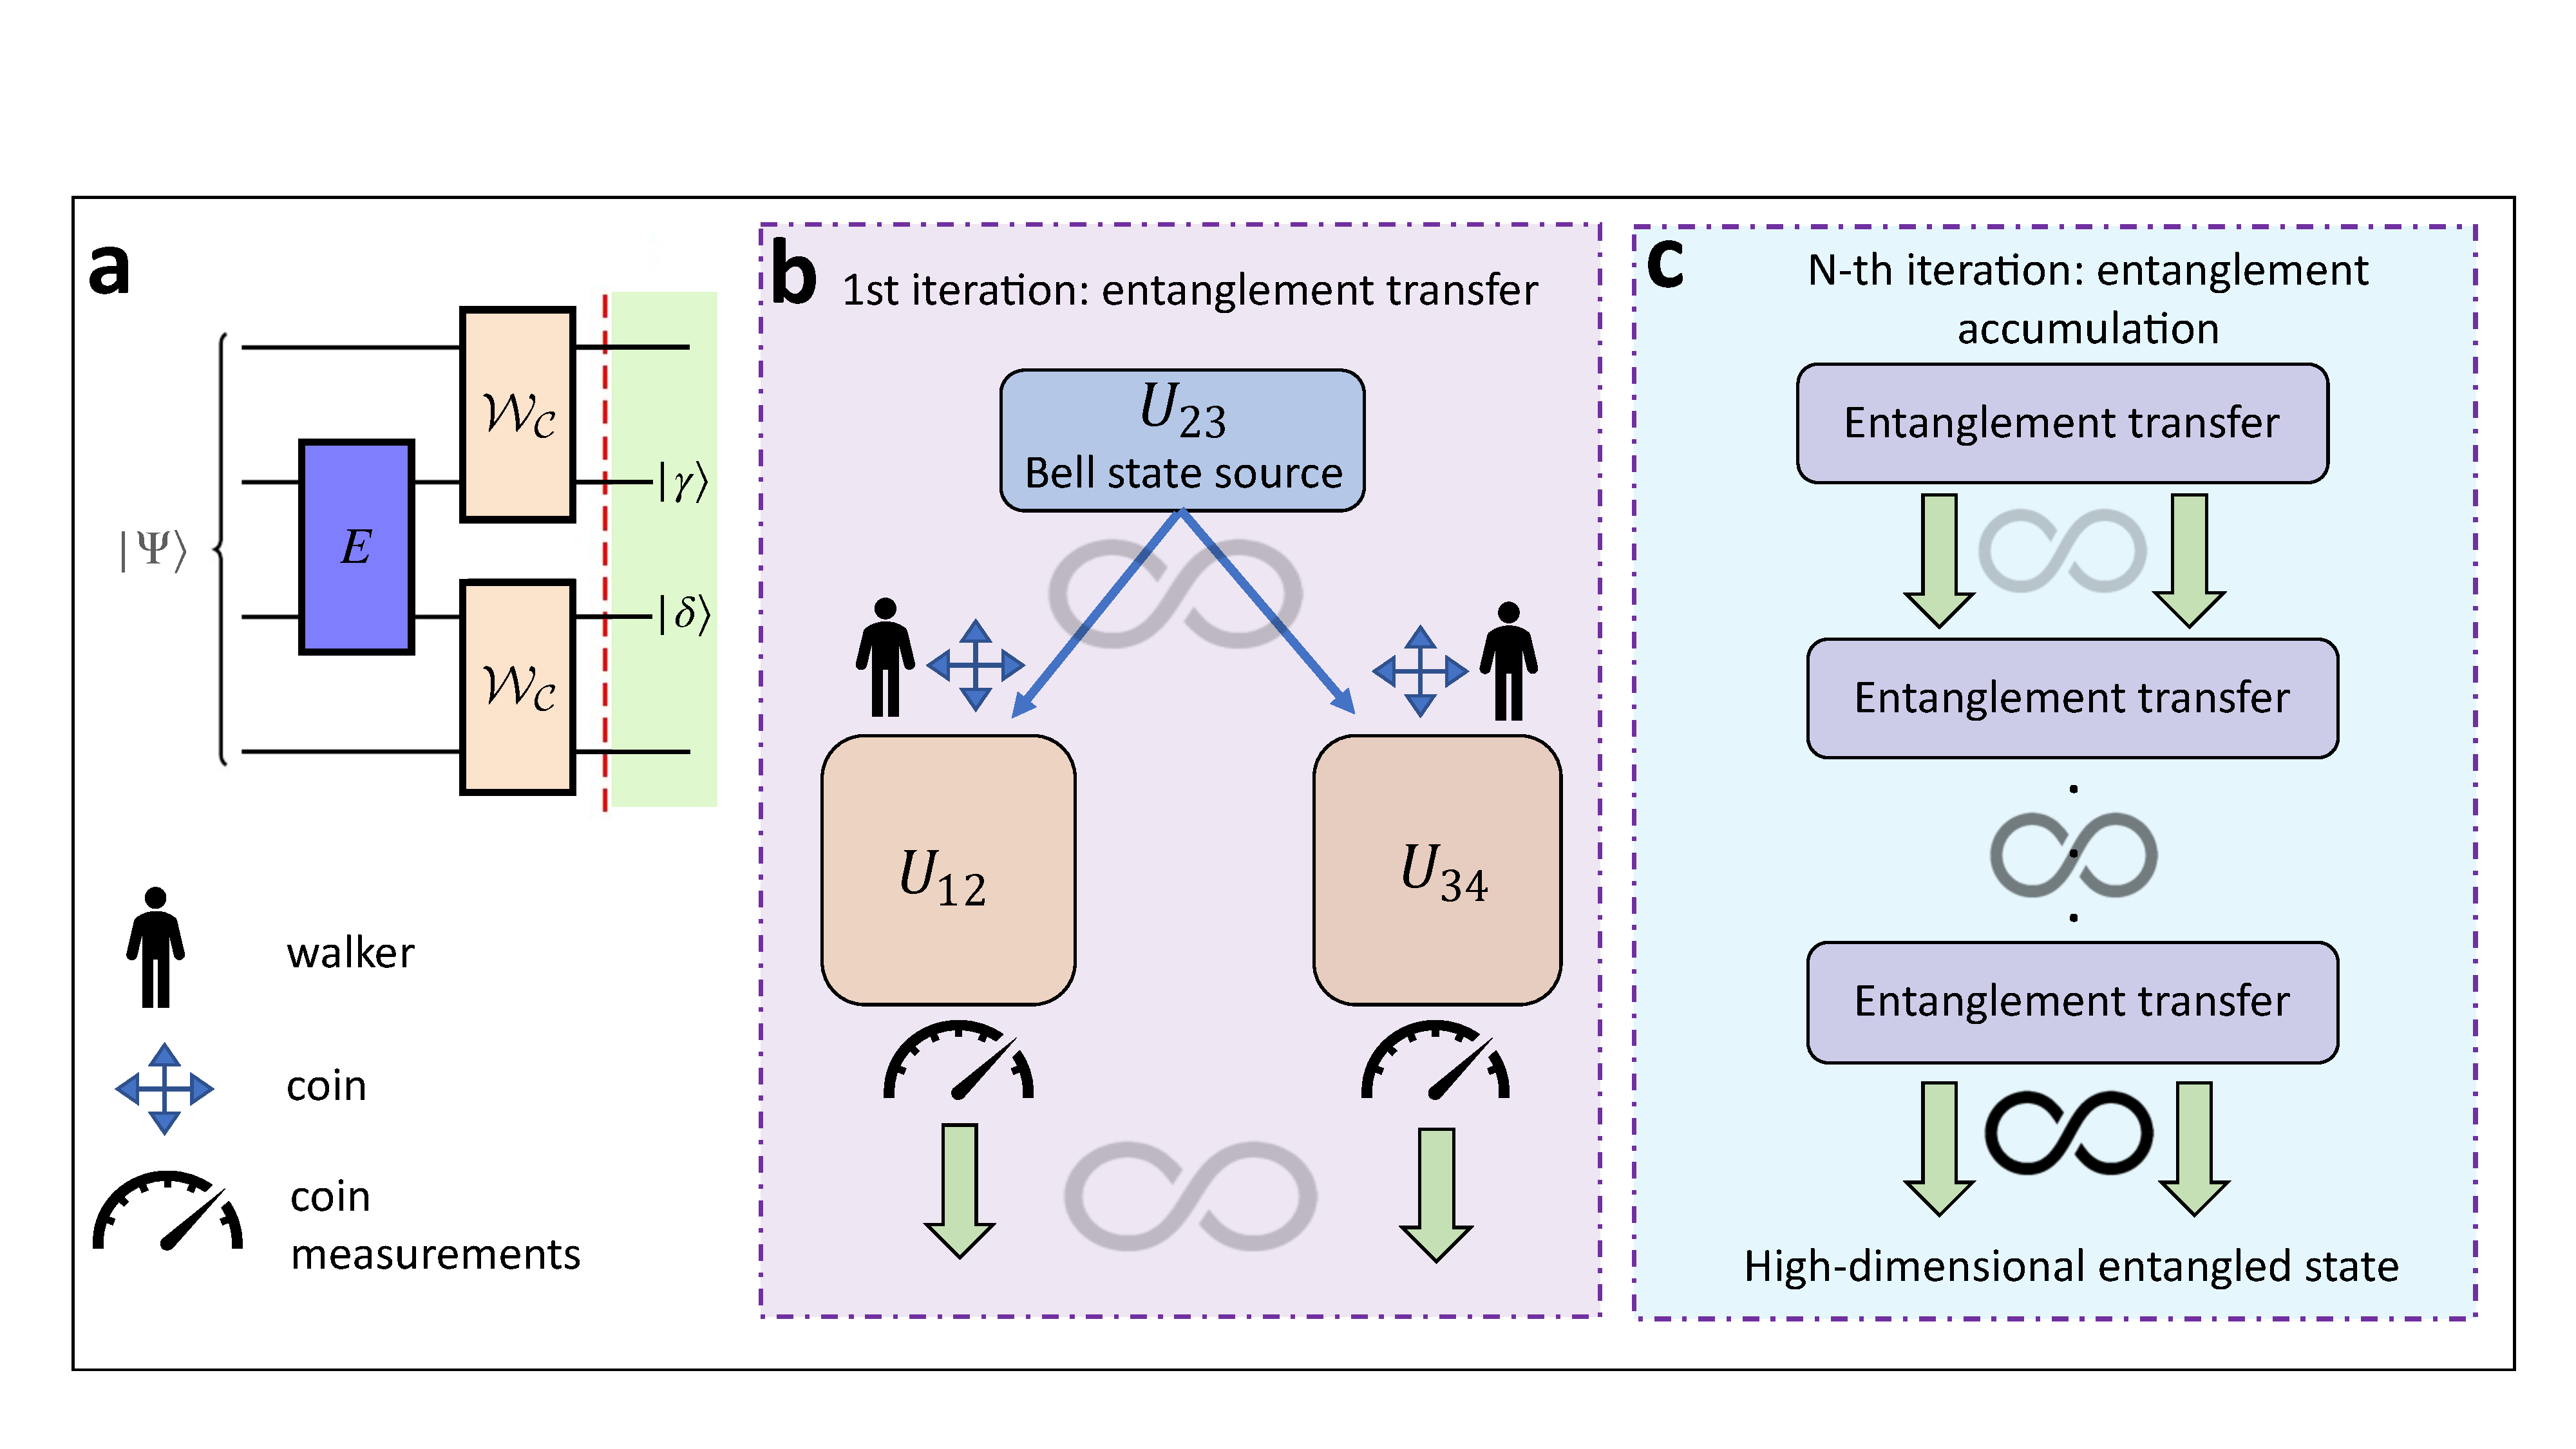
\includegraphics[width=2\columnwidth]{new_conceptMP.pdf}
    \caption{\textbf{Scheme overview.}
        a) Entanglement transfer unit. The system is composed by two particles, 1 and 2, equipped with a $\ell$-dimensional degree of freedom, which will be instrumental to the protocol, and an additional $d$-dimensional degree of freedom. The entanglement transfer protocol requires a first operation $E$ that generates entanglement between the $\ell$-dimensional subsystems. Then we have two {\it local} operations -- with respect to the 1-vs-2 bipartition -- that correlates the inner degrees of freedoms of each particle and realizes the $\ell$-$d$ dynamics. In the end, local measurements allow to transfer the entanglement stored in the initial state to the reduced state of the $d$-dimensional sub-systems. We consider explicitly the case of $\ell=2$ (qubits) and local operations embodied by the walk operations ${\cal W}_{\cal C}$. Indeed, a discrete-time quantum walks framework embodies a very natural encoding of this dynamics: in such embodiment, the  coin particle would embody the $\ell=2$-dimensional system, with the qudit being provided by the position degrees of freedom of the walker. Assuming initially maximally entangled states of the qubits, a single iteration of our protocol would be able to transfer one ebit of entanglement at most. By repeating the use of this unit, high-dimensional entangled states can be generated in the $d$-dimensional degrees of freedom. Furthermore the entanglement stored in such degrees of freedom can be retrieved by same operations and transferred back to the two-qubit state. %A natural encoding of this dynamics can be found within the discrete-time quantum walks framework. Here the quantum walker has the necessary degree of freedom for encoding our protocol, the two dimensional coin and its position spanned on $d$ levels.
         b) Conceptual scheme for the transfer from a Bell state in the coin degree of freedom to the two walkers position space after quantum walks and local coin measurements. c) Protocol iteration and entanglement accumulation in the high-dimensional space of the two quantum walkers.}
    \label{fig:conceptual_scheme}
\end{figure*}

%\parTitle{We use negativity to estimate entanglement}
%\LI{Do we need this paragraph?}
%Throughout this work, in order to discern if a multipartite state is entangled, we will use the PPT criterion (positivity of the partial transpose) \cite{HORODECKI19961}. Such method envisages the calculation of eigenvalues of the partial transpose with respect to one subsystem of the density matrix representing the entire system. If there exists at least one non-positive eigenvalue the state cannot be separable. This criterion is a sufficient condition of non-separability of the multipartite state. Furthermore we can provide an estimation of the amount of entanglement through the state \emph{negativity} $\mathcal{E}_n$ --- \emph{i.e.},  the sum of the negative eigenvalues of the partial transpose density matrix. In the following we make use of the logarithmic negativity defined as $\mathcal{N}=\log_2(2\mathcal{E}_n+1)$. The maximal entanglement reachable in the two-coin subspace is $\mathcal{N}^{Bell}=1$, which is limited by the dimensionality of the coins. In the literature it is common to define such amount of entanglement as \textit{ebit}. In our protocol of entanglement transfer, we then aim at accumulating in the two-walker subspace one ebit of entanglement at most per step of the iterative process mentioned above. This happens only when optimal transfer is achieved, since under operations involving the coins only it is possible at most to transfer the initial value of $\mathcal{N}^{Bell}$.

% \LI{Say later on, when talking about the experiment, something about the photons being non-interacting and the hardness of correlating polarizations etc}

\section{Entanglement transfer via local projections}
\label{sec:entanglement_transfer_local_projections}

\parTitle{Problem statement}
Let us consider the following question
\begin{quote}
% \begingroup\addtolength\leftmargini{-5pt}\begin{quote}
    \textit{Given a four-partite state in $\calH$, can we find local coin projections such that the entanglement in the coin degrees of freedom is transferred to the projected state of the walkers?}
\end{quote}%\endgroup
More precisely, given a state $\ket\Psi\in\calH$, we want to find suitable states $\ket{\gamma}\in\calH^{(1)}_{\calC}$ and $\ket\delta\in\calH^{(2)}_{\calC}$ such that, upon performing {\it bi-local} projections onto them, the coin entanglement possibly present in $\ket\Psi$ is transferred to the projected state
$\braket*{\gamma,\delta}{\Psi}\in\calH^{(1)}_{\calW}\otimes\calH^{(2)}_{\calW}$.
A schematic description of this formal scenario is given in~\cref{fig:conceptual_scheme}a. %\commale{make self-consistent the notation used in the figure and the text ($\ket{\Psi_{in}}$, $\ket{\Psi_{f}}$ and the three unitaries in the figure; in panel (a) it might be worth to put symbols of coin/walker and maybe a curly braket for photon 1 and 2 as well)}.
It is worth stressing that such entanglement transfer is not always possible --- for example if $\ket\Psi$ is trivially separable with respect to the partition $\calH^{(1)}\otimes\calH^{(2)}$: no bilocal operation, including projections, will be able to entangle the walkers. It is therefore pivotal to find the conditions making such protocol viable.

% \begin{figure}
%     \centering
%     \begin{minipage}[c]{\linewidth}
%         \centering
%         \begin{quantikz}
%             \lstick[wires=4]{$\ket{\Psi_{\on{in}}}$}\qw &\qw & \gate[wires=2]{U_{12}}\slice{$\ket{\Psi_f}$} &\qw \\
%             \qw & \gate[wires=2]{U_{23}} & & \qw\rstick{$\!\!\ket{\gamma}$}\\
%             \qw & & \gate[wires=2]{U_{34}} & \qw\rstick{$\!\!\ket{\gamma}$}\\
%             \qw & \qw & \qw & \qw
%         \end{quantikz}
%     \end{minipage}
%     \caption{Entanglement transfer scheme. \highlight{(add decent description)}}
%     \label{fig:entanglement_transfer_scheme}
% \end{figure}

\parTitle{We are actually dealing with two problems at once}
The task at hand can be broken down into two independent sub-problems, which we will refer to as \textit{transferibility conditions}: on the one hand, transferring the entanglement from $\calH^{(1)}_{\calC}\otimes \calH^{(2)}_{\calC}$ to $\calH^{(1)}_{\calW}\otimes \calH^{(2)}_{\calC}$,
and then transferring the entanglement from
$\calH^{(1)}_{\calW}\otimes \calH^{(2)}_{\calC}$
to $\calH^{(1)}_{\calW}\otimes \calH^{(2)}_{\calW}$.
Transferring entanglement from $\calH^{(1)}_{\calC}\otimes\calH^{(2)}_{\calC}$ to
$\calH^{(1)}_{\calW}\otimes\calH^{(2)}_{\calW}$ is possible only if these two sub-problems are solvable.

\parTitle{Conditions for entanglement transfer}
Let $\ket\Psi\in\calH$ have the Schmidt decomposition
\begin{equation}
	\ket\Psi= \sum_k \sqrt{p_k} \ket{u_k}\ket{v_k} 
\end{equation}

with $\sum_k p_k=1$, $\ket{u_k}\in{\cal H}^{(1)}$ and $\ket{v_k}\in{\cal H}^{(2)}$. % and  the corresponding reduced state $\rho\equiv\Tr_2\ketbra\Psi\in\calH^{(1)}$. Projecting onto a coin state $\ket\gamma\in\HC^{(1)}$ then gives $\rho_{\calW}\equiv \mel\gamma\rho\gamma\in\calH^{(1)}_{\calW}$.
We want a projection $\ket\gamma\in\HC^{(1)}$ such that the corresponding post-projection state $\ket{\Psi_\gamma}\in\HW^{(1)}\otimes\calH^{(2)}$ contains the same amount of entanglement, in the bipartition $\HW^{(1)}\otimes\calH^{(2)}$, as that initially in $\ket\Psi$.
In general, we have
\begin{equation}
    \ket{\Psi_\gamma} = \frac{1}{\sqrt{p_{\rm proj}}}
    \sum_k \sqrt{p_k q_k} \ket{\tilde u_k}\ket{v_k},
    \label{eq:postproj_state}
\end{equation}
where
$\sqrt{q_k}\ket{\tilde u_k}= \braket\gamma{u_k}\in{\cal H}^{(1)}$
and
$p_{\rm proj} = \sum_k p_k q_k$.
We distinguish between three different scenarios:
\begin{enumerate}
\item[(1)]If the states $\ket{\tilde u_k}$ are not orthogonal, then some information about which $k$ the state is in leaks through the coin projection, and some  entanglement is thus degraded. This will be shown formally in Appendix~\ref{proof1}.\\
\item[(2)] If the states $\ket{\tilde u_k}$ are orthogonal, but the corresponding projection probabilities $q_k$ are uneven, then again the entanglement in $\ket{\Psi_\gamma}$ is smaller than that in $\ket\Psi$.\\
\item[(3)] If the states $\ket{\tilde u_k}$ are orthogonal, \emph{and} $q_k=p_{\on{proj}}$ for all $k$, \textit{then} projecting onto $\ket\gamma$ fully preserves the initial entanglement.
\end{enumerate}
Note that situation (3) is thus a necessary and sufficient condition for entanglement transferability without degradation,
as if $\braket{\tilde u_j}{\tilde u_k}=\delta_{jk}$ and $q_k=p_{\on{proj}}$ then~\cref{eq:postproj_state} is the Schmidt decomposition of $\ket{\Psi_\gamma}$, and therefore the Schmidt coefficients of $\ket{\Psi_\gamma}$ are (in the relevant bipartition) the same as those of $\ket{\Psi}$.
% Note that, if the projection probabilities $q_k$ are the same for all $k$, then $q_k=p                                                                          _{\rm proj}$ and thus $\ket{\Psi_\gamma}$ displays the same entanglement as $\ket{\Psi}$:
% \begin{equation}
%     \ket{\Psi_\gamma} = \sum_k \sqrt{p_k} \ket{\tilde u_k}\ket{v_k}.
% \end{equation}
% More precisely, if $\bs p$ and $\bs p'$ are the vectors of squares of the Schmidt coefficients before and after the projection, respectively, then $\bs p'\prec\bs p$, and thus the amount of entanglement in $\ket{\Psi_\gamma}$ is less than that in $\ket\Psi$~\cite{nielsen1999conditions}.
% It follows that a necessary condition for optimal transferability is that $q_k=p_{\on{proj}}$, \textit{i.e.} that all components of $\ket{\Psi}$ have the same squared overlap with $\ket\gamma$. This condition is however not sufficient.

%TESTO SPOSTATO IN APPENDICE A

\parTitle{Summary of conclusions}
Therefore, we achieve transferability if $\ket\gamma$ is such that
$\braket{\gamma}{u_k}/{\sqrt{p_{\on{proj}}}}$ are orthonormal vectors.
An equivalent -- if less explicit -- condition for transferability is to require that% nonzero spectrum of $\tr_2(\PP_{\Psi_\gamma})$ be the same as the nonzero spectrum of $\tr_2(\PP_\Psi)$:
\begin{equation}
    % \frac{1}{p_{\on{proj}}} \tilde\sigma\left(
    %     \langle\gamma\rvert \tr_2(\PP_\Psi)\lvert \gamma\rangle
    % \right) =
    \tilde\sigma(\tr_2(\PP_{\Psi_\gamma})) =
    \tilde\sigma\left(
        \tr_2(\PP_\Psi)
    \right),
    \label{eq:transferability_condition}
\end{equation}
where $\tilde\sigma(A)\equiv\sigma(A)\setminus\{0\}$ and $\sigma(A)$ is the set of eigenvalues of $A$.
This is a \emph{necessary and sufficient} condition for transferability, as~\cref{eq:transferability_condition} is equivalent to requesting that the Schmidt coefficients of $\ket{\Psi_\gamma}$ are the same as those of $\ket{\Psi}$.
We will refer to~\cref{eq:transferability_condition} as the \emph{first transferability condition} ($\on{TC}_1$), in that it characterises the transferability of the entanglement with respect to the bipartition $\calH^{(1)}\otimes\calH^{(2)}$ into entanglement with respect to the bipartition $\HC^{(1)}\otimes\calH^{(2)}$.
%In other words, \eqref{eq:transferability_condition} is a necessary and sufficient condition to ensure that the correlations between $\calH^{(1)}$ and a second party can be \emph{offloaded} onto $\HW^{(1)}$ by means of a local projection.
The analogous condition on the second party, involving finding a suitable projection $\ket\delta\in\HC^{(2)}$, will be denoted with $\on{TC}_2$.
Entanglement transfer is therefore achievable if and only if $\on{TC}_1$ \emph{and} $\on{TC}_2$ are satisfied.
In~\cref{fig:TC1_general_condition_scheme,fig:TC1_condition_scheme} we present a pictorial description of what $\on{TC}_1$ allows to achieve.
It is worth noting that, while~\cref{eq:transferability_condition} is required to fully transfer entanglement, it is still possible to transfer \textit{some} degree of entanglement as long as the vectors  $\braket{\gamma}{u_k}$ are orthogonal, even though the projection probabilities are unequal.

% This ensures that the projection does not reveal any information about the correlations with $\calH^{(2)}$, which would damage the entanglement.
% More explicitly, this ensures that the state, written in Schmidt form with respect to the bipartition $\calH^{(1)} \otimes \calH^{(2)}$,
% \begin{equation}
% 	\ket\Psi= \sum_k \sqrt{p_k} \ket{u_k}\ket{v_k} \;, 
% \end{equation}
% with $\ket{u_k} \in \calH^{(1)}$ and $ \ket{v_k} \in \calH^{(2)}$, becomes
% \begin{equation}
% 	\braket{\gamma}{\Psi} =
% 	\sqrt{p_{\on{proj}}}\sum_k \sqrt{p_k} \ket*{\tilde u_k}\ket{v_k}\;,
% \end{equation}
% where $\ket*{\tilde u_k}\equiv \braket{\gamma}{u_k}/\sqrt{p_{\on{proj}}} \in\calH^{(1)}_{\calW}$ are the post-projected states, and
% $p_{\on{proj}}\equiv |\braket{\gamma}{u_k}|^2$ the projection probability.
% It is worth stressing that, \emph{a priori}, the projection probabilities $|\braket{\gamma}{u_k}|^2$ depend on $k$, but we need them to be the same for optimal entanglement transfer.
% The constraint on the projection probabilities can be lifted when the projection allowed in the second party is taken into consideration.
% This is because any form of ``imperfect entanglement'' can be improved by means of local projections in some cases (\emph{i.e.} local projections are sufficient to transform a state of the form $\sum_k \sqrt{p_k}\ket{u_k}\ket{v_k}$ into the corresponding maximally entangled state $\sum_k \ket{u_k}\ket{v_k}$).\LI{probably lose the paragraph above}

\parTitle{Relations with entanglement swapping}
This problem can be understood as a more restrictive version of entanglement swapping.
Such protocol~\cite{zukowski1993eventreadydetectors} deals with a four-partite system in the Hilbert space $\otimes_{j}\calH_{j}~(j=A,B,C,D)$, whose state is  separable in the bipartition $(AB)$-vs-$(CD)$ but entangled in the subsystems $A-B$ {\it and} $C-D$. The goal of entanglement swapping is to achieve  entanglement in the state of the $A-D$ compound by performing projective measurements on $B-C$. This is possible for instance by implementing a Bell measurement over the joint state of $B$ and $C$. Clearly, the problem is analogous to ours, except that we only allow \emph{local} operations on $B$ and $C$. Notably, the use of a Bell measurement is not available in our setting.

\begin{figure}[b]
    \centering
    \includestandalone[width=\columnwidth]{tikz-figures/TC1_general}
    \caption{Pictorial representation of the first transferability procedure.
    Given a state which is entangled with respect to the bipartition $\calH^{(1)}\otimes\calH^{(2)}$, we apply a local projection $\ket\gamma$ which preserves the entanglement between the two spaces.
    Condition~\eqref{eq:transferability_condition} determines when such a projection exists.
    }
    \label{fig:TC1_general_condition_scheme}
\end{figure}

\begin{figure}[b]
    \centering
    \includestandalone[width=\columnwidth]{tikz-figures/TC1}
    \caption{
        Like~\cref{fig:TC1_general_condition_scheme}, but for states in which the entanglement is only due to pre-shared entanglement between the coins. These are the types of states at the first entanglement accumulation step.
    }
    \label{fig:TC1_condition_scheme}
\end{figure}

\section{Entanglement transfer through Quantum-Walk dynamics}
\label{sec:entanglement_transfer_in_QWs}

In~\cref{sec:entanglement_transfer_local_projections} we discussed the general problem of transferring entanglement by means of local projections.
Most notably we made no assumption on the inner structure of correlations in $\calH^{(i)}$, nor we specified the dimensionality of the entanglement in the bipartition $\calH^{(1)}\otimes\calH^{(2)}$. The framework and results set up so far thus also apply to %subsequent iterations of entanglement accumulation, and more generally 
cases where some pre-existing entanglement exists between the walkers' degrees of freedom.
We now specialize our study to the case $\dim\HC^{(i)}=2$, which applies directly to QWs with two-dimensional coins.
More precisely, in~\cref{subsec:generalsolution_firstiteration_2Dcoin} we consider states in which $\calH^{(1)}$ and $\calH^{(2)}$ are only entangled through their coin spaces (as in~\cref{fig:TC1_condition_scheme}).
In~\cref{subsec:analytical_results_QWs} we then apply these results to the output states obtained from the QW dynamics.
Finally, we present a numerical study illustrating the implications of our analytical results.
% \begin{figure}
%     \centering
%     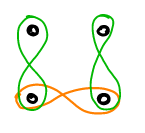
\includegraphics[width=0.6\linewidth]{figures/ent_structure_drawing.png}
%     \caption{Awesome entanglement structure representation}
%     \label{fig:ent_structure_representation}
% \end{figure}

\subsection{Entanglement transfer via two-dimensional coins}
\label{subsec:generalsolution_firstiteration_2Dcoin}

\parTitle{Problem setting}
Consider a state $\ket\Psi\in\calH^{(1)}\otimes\calH^{(2)}$ which is entangled only via its coin spaces, as in~\cref{fig:TC1_condition_scheme}. The corresponding reduced state %$\rho\in\mathrm{Lin}(\calH^{(1)})$ 
reads
\begin{equation}
	\rho= p_1 \PP_u + p_2 \PP_v, \,\,p_1+p_2=1,
	\label{eq:reduced_state_twodimcase}
\end{equation}
for a pair of orthonormal states $\{\ket u,\ket v\}\in\calH^{(1)}$.
To highlight the entanglement in $\HC^{(1)}\otimes\HW^{(1)}$, we can write these states as
\begin{equation}
\begin{aligned}
    \ket u &=
    \cos(\theta_u) \ket{\uparrow, u_\uparrow} +
    \sin(\theta_u) \ket{\downarrow, u_\downarrow}, \\
    \ket v &=
    \cos(\theta_v) \,\ket{\uparrow, v_\uparrow} +
    \sin(\theta_v) \ket{\downarrow, v_\downarrow}.
\end{aligned}
\end{equation}
As discussed in~\cref{sec:entanglement_transfer_local_projections}, to achieve maximal entanglement transfer we need a projection onto a state $\ket\gamma$ satisfying $\on{TC}_1$, i.e. fulfilling~\cref{eq:transferability_condition}.
This is equivalent to requiring $\braket{\tilde u}{\tilde v}=0$ where $\braket{\gamma}{j}=\sqrt{p_{\on{proj}}}\ket{\tilde j}~(j=u,v)$.
Explicitly, these amount to the conditions
\begin{equation}
	\mel{\gamma}{\tr_{\calW}(\ketbra{u}{v})}{\gamma} = 0,
\end{equation}
and
$\mel{\gamma}{\tr_{\calW}(\ketbra{u})}{\gamma} =
\mel{\gamma}{\tr_{\calW}(\ketbra{v})}{\gamma} = p_{\on{proj}}$.

In Appendix~\ref{appB} we demonstrate that, when the entanglement in the bipartition $\calH^{(1)}\otimes\calH^{(2)}$ is two-dimensional and thus the reduced state can be written as in~\cref{eq:reduced_state_twodimcase}, it is always possible to find a projection onto a state $\ket\gamma$ preserving orthogonality.
To fully satisfy condition $\on{TC}_1$, one then only has to verify that the projection probabilities are equal.

\subsection{Entanglement transfer with coined QWs}
\label{subsec:analytical_results_QWs}
% \commale{introduce what this subsection/section is about and how it is structured: 1 step, n steps, pairs of QW analytically but for 1 step only, pairs of QW numerically for n steps?}

\parTitle{Section outline}
We now apply the results of the previous section to the specific quantum states resulting from coined QWs.
As in~\cref{subsec:generalsolution_firstiteration_2Dcoin}, we first %focus on the reduced state in $\calH^{(1)}$ and on its satisfying $\on{TC}_1$, to then show how to study the full system, to ensure the satisfiability of both $\on{TC}_1$ and $\on{TC}_2$. More specifically, we 
assume that the overall state is entangled with respect to the bipartition $\calH^{(1)}\otimes\calH^{(2)}$ only via its coin spaces, as in~\cref{fig:TC1_condition_scheme} and~\cref{sec:entanglement_transfer_in_QWs}. We thus take the initial full state of the form
\begin{equation}
\ket{\Psi}=    \sqrt{p_1} \ket{\uparrow,1}\otimes\ket{\uparrow,1} +
    \sqrt{p_2} \ket{\downarrow,1}\otimes\ket{\downarrow,1},
\end{equation}
for some coefficients $p_1,p_2\ge0$ with $p_1+p_2=1$.
Focusing on $\calH^{(1)}$, we thus see that the initial states upon which the QW operates are $\ket{\uparrow,1}$ and $\ket{\downarrow,1}$.

\parTitle{Single step}
A single QW step with coin operation  ${\cal C}$ %\equiv (c_{ij})_{ij}$ 
amounts to the evolution
\begin{equation}
\begin{aligned}
	\ket{\uparrow,1} &\rightarrow \ket*{\Psi_{\uparrow,1}} \equiv c_{11}\ket{\uparrow,1} + c_{21}\ket{\downarrow,2}, \\
	\ket{\downarrow,1} &\rightarrow \ket*{\Psi_{\downarrow,1}} \equiv c_{12}\ket{\uparrow,1} + c_{22}\ket{\downarrow,2},
\end{aligned}
\end{equation}
where $c_{ij}$ are the entries of the unitary matrix representing ${\cal C}$. By projecting onto $\ket\gamma\equiv \gamma_\uparrow\ket\uparrow+\gamma_\downarrow\ket\downarrow~(\gamma_{\uparrow,\downarrow}\in\mathbb{C})$ and imposing %we get
%\begin{equation}
%\begin{aligned}
%	\ket*{\psi_\uparrow} \equiv  \braket*{\gamma}{\Psi_{\uparrow,1}} &= \gamma_\uparrow^*c_{11}\ket1 + \gamma_\downarrow^* c_{21}\ket2, \\
%	\ket*{\psi_\downarrow} \equiv  \braket*{\gamma}{\Psi_{\downarrow,1}} &= \gamma_\uparrow^* c_{12} \ket1 + \gamma_\downarrow^* c_{22} \ket2.
%\end{aligned}
%\end{equation}
the orthogonality condition of the reduced states, we get%then reads
\begin{equation}
\begin{gathered}
%	\braket*{\psi_\uparrow}{\psi_\downarrow}=
	% \mel{\gamma}{\tr_{\calW}(\ketbra*{\Psi_\uparrow}{\Psi_\downarrow})}{\gamma}
	 |\gamma_\uparrow|^2 c_{11}^* c_{12} + |\gamma_\downarrow|^2 c_{21}^* c_{22} = 0,
\end{gathered}
\end{equation}
which is satisfied if $\ket\gamma = (\ket\uparrow + e^{i\phi}\ket\downarrow)/\sqrt2$ for any $\phi\in\RR$, consistently with~\cref{eq:definition_projgamma_2dcase}.
The corresponding projection probabilities are both equal to $1/2$, as follows from
\begin{equation}
\begin{aligned}
	2\abs{\braket{\gamma}{\Psi_{\uparrow,1}}}^2 &= |c_{11}|^2 + |c_{21}|^2 = 1, \\
	2\abs{\braket{\gamma}{\Psi_{\downarrow,1}}}^2 &= |c_{12}|^2 + |c_{22}|^2 = 1.
\end{aligned}
\end{equation}
We conclude that $\on{TC}_1$ is always achievable for this class of states.
% More precisely, if the initial state $\ket*{\Psi_{\on{in}}}$ of the QW  is entangled via its coin with an external degree of freedom, as in
% \begin{equation}
% 	\sqrt2\ket*{\Psi_{\on{in}}} = \ket{\uparrow,1} \otimes \ket{u_1} + \ket{\downarrow,1}\otimes \ket{u_2},
% \end{equation}
% with $\ket{u_i}$ arbitrary orthogonal states \commale{orthogonality is non-general but crucial for us, stress this?} of the additional degree of freedom,
% then the entanglement can always be transferred from $\calH_{\calC}$ to $\calH_{\calW}$ with probability $1/2$.
Remarkably, the freedom in the choice of the phase $\phi$ means that projections onto $\ket\pm= (\ket\uparrow+\ket\downarrow)/\sqrt2$ (as well as any other orthonormal basis of balanced states) are suitable to achieve entanglement transfer.
This results in an overall transfer success probability of $1$: measuring in the $\ket\pm$ basis, both of the possible outcomes achieve $\on{TC}_1$, albeit with different post-projection states.

\parTitle{Multiple steps}
Consider now the state after multiple QW steps.
%Denoting with $\calU$ the unitary evolution implemented by the QW, and 
%Assuming the initial coin states to be $\ket\uparrow$ and $\ket\downarrow$, 
The final reduced state on $\calH^{(1)}$ is a mixture of $\ket{\Psi_\uparrow}$ and $\ket{\Psi_\downarrow}$, where
% \commale{same as above, fix the notation (coin as first or second argument, consistently); is the index $s$ standing for $s$-th step?}
\begin{equation}
\begin{aligned}
	\ket{\Psi_s} =
	\cos(\theta_s) \ket{\uparrow,\Psi_{s,\uparrow}} +
	\sin(\theta_s) \ket{\downarrow,\Psi_{s,\downarrow}},
	% s\in\{\uparrow,\downarrow\}.
\end{aligned}
\end{equation}
with $\theta_s$ and $\ket{\Psi_{s,p}}$ depending on the number of steps and choice of coin operators, and $s,p\in\{\uparrow,\downarrow\}$.
To assess the achievability of $\on{TC}_1$ we consider, as in~\cref{subsec:generalsolution_firstiteration_2Dcoin}, the matrix
$M\equiv \tr_{\calW}(\ketbra{\Psi_\uparrow}{\Psi_\downarrow})$.
This has the form
\begin{equation}\scalebox{0.97}{$\displaystyle
	M = \begin{pmatrix}
		\cos(\theta_\uparrow)\cos(\theta_\downarrow) \calO_{\uparrow\uparrow} &
		\cos(\theta_\uparrow)\sin(\theta_{\downarrow}) \calO_{\downarrow\uparrow} \\
		\cos(\theta_\downarrow)\sin(\theta_{\uparrow}) \calO_{\uparrow\downarrow} &
		\sin(\theta_\uparrow)\sin(\theta_\downarrow) \calO_{\downarrow\downarrow}
	\end{pmatrix}.
$}\end{equation}
with
$\calO_{sp}\equiv\braket{\Psi_{\downarrow s}}{\Psi_{\uparrow p}}$.
Matrix $M$ is not in general Hermitian, nor normal. Consequently, while it is possible to find a state $\ket\gamma$ upon which to perform a projection [cf.~\cref{eq:definition_projgamma_2dcase}], the corresponding projection probabilities are not in general equal. We show two cases in which there is no such $\ket\gamma$ in~\cref{fig:contourPlot_overlapAndEntropies_rnd4steps,fig:contourPlot_overlapAndEntropies_Hadamard4steps}.
In general, random QW evolutions with more than one step always correspond to a behaviour akin to this one:%~\cref{fig:contourPlot_overlapAndEntropies_rnd4steps,fig:contourPlot_overlapAndEntropies_Hadamard4steps}, that is, to there being 
no $\ket\gamma$ exists enabling the fulfillment of both the conditions required to achieve $\on{TC}_1$.

However, there are still many cases in which $\on{TC}_1$ is achievable. For example, consider a QW in which the coin is always taken to be identity: ${\cal C}=I$ at all steps. Then, after $n$ steps, the dynamics amounts to
\begin{equation}
    \ket{\uparrow,1} \to \ket{\uparrow, 1}, \quad
    \ket{\downarrow,1} \to \ket{\downarrow, n},
\end{equation}
where $\ket k$ denotes the $k$-th walker position.
The matrix $M$ is thus in this case easily seen to be $M=0$, implying that the orthogonality requirement is always satisfied, making $\on{TC}_1$ achievable as long as the projection probabilities are equal. This constraint is satisfied by any balanced projection of the form $\ket\gamma=(\ket0+e^{i\phi}\ket1)/\sqrt2$, $\phi\in\RR$.

% This can be fixed by either choosing coin operations which make these probabilities equal, when that is possible, or by compensating unequal projection probabilities with similar projection probabilities on the other party \commale{do we show this explicitly?}.

\begin{figure}[tb]
    \centering
    \begin{tikzpicture}
		\node[anchor=south west] (A) at (0, 0)%
			{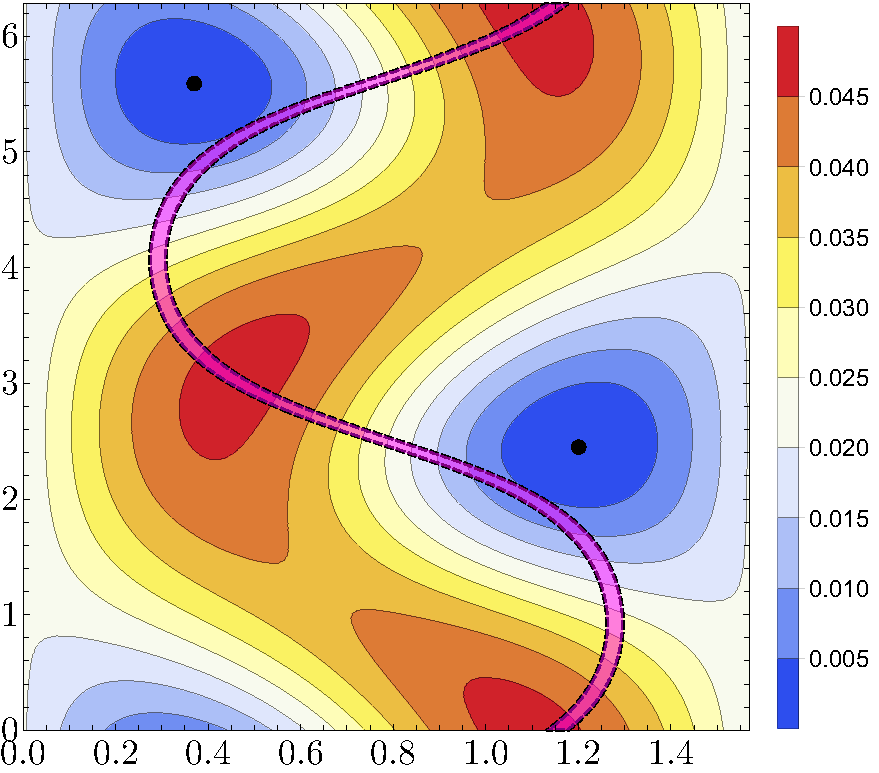
\includegraphics[width=0.9\linewidth]{figures/contourPlot_overlaps_withMaxEntropyRegion_rnd4steps.pdf}};
		\node[above] at (3.6, -.3) {$\theta$};
		\node[above] at (-.2, 3.4) {$\phi$};
	\end{tikzpicture}
    \caption{Final overlap and projection probabilities for the different possible projections $\ket\gamma=\cos(\theta)\ket0+\sin(\theta)e^{i\phi}\ket1$, for the output of a random QW with $4$ steps.
    More precisely, we consider a QW evolution $\calU$ composed of four steps with four random coin operations.
    We then consider the input states $\ket{\Psi_\uparrow}\equiv\calU\ket{\uparrow,1}$ and $\ket{\Psi_\downarrow}\equiv\calU\ket{\downarrow,1}$.
    For each, we verify the satisfiability of $\on{TC}_1$.
    For the purpose, we first plot the squared overlap $\|\braket{\Psi_\uparrow}{\gamma}\braket{\gamma}{\Psi_\downarrow}\|^2$ for all possible $\ket\gamma$.
    We find that there are two orthogonal projections $\ket{\gamma_1},\ket{\gamma_2}$ such that this quantity is zero, represented in the figure with black dots.
    As discussed in~\cref{sec:entanglement_transfer_local_projections}, the vanishing overlap is only a necessary, not sufficient condition. To achieve $\on{TC}_1$, we also require the projection probabilities being equal: $p_\uparrow=p_\downarrow$ where $p_s\equiv \|\braket{\Psi_s}{\gamma}\|^2$, $s\in\{\uparrow,\downarrow\}$.
    In the plot, we represent the values of $(\theta,\phi)$ for which this condition is satisfied with the magenta region bounded by dashed black lines.
    More precisely, the magenta region outlines the set of $(\theta,\phi)$ such that the entropy of the projections probabilities, $S((p_\uparrow, p_\downarrow))$, is larger than $0.693$ (remembering that $-\ln2\simeq 0.6931$).
    It is worth noting that, while it is not in general true that $p_\uparrow+p_\downarrow$ for an arbitrary unitary evolution, this is always the case for QW evolutions, which allows us to quantify how close $p_\uparrow$ and $p_\downarrow$ via the corresponding entropy.
    As clear from the figure, $\on{TC}_1$ cannot be achieved for any $\ket\gamma$, as the two necessary conditions cannot be simultaneously satisfied.
    }
    \label{fig:contourPlot_overlapAndEntropies_rnd4steps}
\end{figure}

\begin{figure}[tb]
    \centering
    \begin{tikzpicture}
		\node[anchor=south west] (A) at (0, 0)%
			{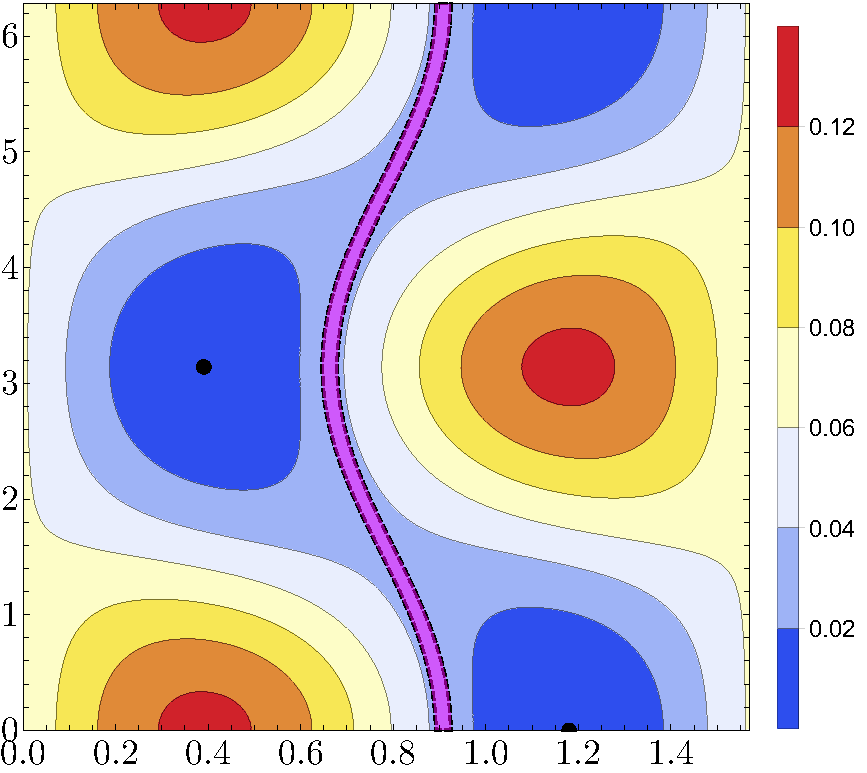
\includegraphics[width=0.9\linewidth]{figures/contourPlot_overlaps_withMaxEntropyRegion_Hadamard4steps.pdf}};
		\node[above] at (3.6, -.3) {$\theta$};
		\node[above] at (-.2, 3.4) {$\phi$};
	\end{tikzpicture}
    \caption{Same as~\cref{fig:contourPlot_overlapAndEntropies_rnd4steps} but for a four-step Hadamard walk.
    As was the case for random QWs, we see that the two requirements to achieve $\on{TC}_1$ are incompatible (the magenta region bounded by dashed lines does not cross the black dots).
    }
    \label{fig:contourPlot_overlapAndEntropies_Hadamard4steps}
\end{figure}


%\parTitle{Pair of QWs}
%\LI{we could also remove this paragraph. I don't think it adds much, but let me know what you think}
%Consider now a pair of coins in an entangled state
%\begin{equation}
%	\sqrt2\ket{\Psi_{\calC}}\equiv \ket{\uparrow,\downarrow} + \ket{\downarrow,\uparrow}.
%\end{equation}
%Assuming the walkers are initially not entangled, the full initial state $\ket{\Psi_{\on{input}}}$ satisfies
%\begin{equation}
%    \tr_\calC(\PP_{\Psi_{\on{input}}}) = 
 %   \ket*{\Psi_\calW^{(1)}} \otimes
%    \ket*{\Psi_\calW^{(2)}} \in \HW^{(1)}\otimes\HW^{(2)}.
%\end{equation}
%Applying the same QW evolution $\calU_{\on{QW}}$ on both $\calH^{(1)}$ and $\calH^{(2)}$, the output state reads
%\begin{equation}
%	\sqrt2(\calU_{\on{QW}}\otimes \calU_{\on{QW}})
%	\ket{\Psi_{\on{input}}} =
%	\ket{\Psi_\uparrow,\Psi_\downarrow} +
%	\ket{\Psi_\downarrow,\Psi_\uparrow},
%\end{equation}
%for some $\ket*{\Psi_\uparrow},\ket{\Psi_\downarrow}\in\calH^{(i)}$ which depend on the choice of $\calU_{\on{QW}}$.
%The reduced states on $\calH^{(1)}$ and $\calH^{(2)}$ are thus both equal to
%% \begin{equation}
%	$2\rho = \PP_{\Psi_\uparrow} + \PP_{\Psi_\downarrow}$,
%% \end{equation}
%and the transferability conditions amount to
%\begin{equation}
%	\mel{\gamma}{\tr_{\calW}(\ketbra{\Psi_\uparrow}{\Psi_\downarrow})}{\gamma} = 0.
%\end{equation}
%We can always find two orthogonal projections $\ket{\gamma_i}$, $i=1,2$ that satisfy this condition, as shown previously.
%Fixing one of these, the post-selected state is
%\begin{equation}
%	\braket*{\gamma^{(1)}}{\Psi_\uparrow}\otimes \braket*{\gamma^{(2)}}{\Psi_\downarrow}
%	+
%	\braket*{\gamma^{(1)}}{\Psi_\downarrow}\otimes \braket*{\gamma^{(2)}}{\Psi_\uparrow},
%\end{equation}
%with $\ket*{\gamma^{(i)}}$ the projection used on the $i$-th QW.
%For the resulting state to be maximally entangled we need
%\begin{equation}\scalebox{0.96}{$\displaystyle
%	\|\braket*{\gamma^{(1)}}{\Psi_\uparrow}\|
%	\|\braket*{\gamma^{(2)}}{\Psi_\downarrow}\|
%	=
%	\|\braket*{\gamma^{(1)}}{\Psi_\downarrow}\|
%	\|\braket*{\gamma^{(2)}}{\Psi_\uparrow}\|.
%$}\end{equation}
%This can be satisfied by choosing $\ket*{\gamma^{(1)}}=\ket*{\gamma^{(2)}}$, or alternatively if the projection probabilities corresponding to $\gamma^{(1)}$ and $\gamma^{(2)}$ are the same.
%We have for example the latter case when using a single QW step.
%The entanglement transfer scheme then becomes deterministic, as any outcome of the coin measurement leads to the entanglement being transferred from coin to walker degree of freedom.

%% Suppose the two photons are initially the state
%% \begin{equation}
%%     \ket{\on{initial}}\equiv
%%     (a_{p_0,\ell_0,H}^\dagger
%%     a_{p_1,\ell_0,V}^\dagger +
%%     a_{p_0,\ell_0,V}^\dagger
%%     a_{p_1,\ell_0,H}^\dagger) \ket{\mathrm{vac}},
%%     \label{eq:proj_initial_state}
%% \end{equation}
%% for some initial OAM $\ell_0$, and with $p_i, i=0,1$ the $i$-th position.
%% Note that~\cref{eq:proj_initial_state} is nothing but a state of the form $\ket{HV}+\ket{VH}$ in second quantisation notation.
%% As long as no operation interfering the two photons is used, we can safely operate in this bra-ket notation.
%% Evolving the photons locally with the same unitary $\calU$ gives
%% $(\calU\otimes\calU)(\ket{HV}+\ket{VH})$.
%% Let us then define
%% $\ket{\Psi^s}\equiv\calU\ket s$, with $s\in\{H,V\}$.
%% The states $\ket{\Psi^s}$ are one-photon states which in general display entanglement between their polarisation and OAM degrees of freedom:
%% \begin{equation}
%%     \ket{\Psi^s}=
%%     \cos\theta_s \ket H\otimes\ket{\Psi^s_{H}} +
%%     \sin\theta_s \ket V\otimes\ket{\Psi^s_{V}},
%% \end{equation}
%% for some angle $\theta_s$ and states $\ket{\Psi^s_p}$.

%\subsection{Numerical Results}
%\label{subsec:numerical_results_QWs}

%\LI{should we merge this into subsection B? Knowing that $C=I$ works makes these numerics less justified, though they might still be of interest}

\parTitle{What do we do here and why}
As discussed above, whereas the output of a single QW step always allows for optimal transferability, this is not always the case for the output of multiple steps.
We now present numerical results exploring the satisfiability of $\on{TC}_1$ for these states.
% Let us now focus on the task of transfering entanglementfrom the states of two maximally entangled qubits to two qudits states via local quantum walks routine and suitable coin projections. In the previous sections, it has been shown that this two local projectors can be found regardless the choice of the QW routines $\mathcal{U}$ and $\mathcal{V}$. Here we provide some numerical results that confirm such intuition
% Given a basis $b = \{\ket{\gamma_0},\ket{\gamma_1}\}$ for the coin degree of freedom, consider the associated projectors
% $\PP_{ij}\equiv \ketbra{\gamma_i}\otimes\ketbra{\gamma_j}$. 
% For an input state of the two quantum walks of the form
% $\ket{\Psi^{in}}=\frac{1}{\sqrt{2}}(\ket{\uparrow,\downarrow}+\ket{\downarrow,\uparrow})\otimes \ket{0,0}$ \commale{make notation consistent} we obtain as output
% $\ket{\Psi^{out}}=\alpha\ket{\Psi_\uparrow\Psi_\downarrow}+\beta\ket{\Psi_\downarrow\Psi_\uparrow}$. Applying the projectors $\PP_{ij}$ to the final state we get
% we get
% \begin{equation}
%     \alpha\ket*{\psi_\uparrow^i\psi_\downarrow^j} +
%     \beta\ket*{\psi_\downarrow^i\psi_\uparrow^j}.
%     \label{eq:qudit_ent}
% \end{equation}
\parTitle{Case with same QW on both sides}
In Fig. \ref{fig:10steps_results} we report the logarithmic negativity $\mathcal{N}$ and the associated projection probabilities expressed in terms of the parameters that define the states upon which the projections are performed. These are expressed as $\ket{\gamma_0}\equiv\cos{\frac{\theta}{2}} \ket{\uparrow}+ 
 \mathrm{e}^{\mathrm{i}\phi}\sin{\frac{\theta}{2}}\ket{\downarrow}$ and $\gamma_1$ as the orthogonal,
where $\theta \in [0, \pi ]$ and $\phi \in [0, 2\pi]$. In this simulations we consider for simplicity two identical Hadamard QWs, i.e biased coin operators, of 10 steps \commale{why are we doing this if 1 step is sufficient for complete transfer? Don't we actually loose from this, in terms of probability}. It is worth to note that it possible to find regions with high projection probability and log-negativity. Here the maximum value reachable is fixed by the initial state, which has log-negativity 1. The projection probabilities of such two-qudit states in eq.\eqref{eq:qudit_ent} can be even bigger than the values reported in Fig.\ref{fig:10steps_results}c-d, since the projectors $\PP_{11}$ and $\PP_{10}$ generates states with the same log-negativity reported in Fig.\ref{fig:10steps_results}.
Equivalent results can be retrieved for any QWs and number of steps, confirming the results of the analytical description \commale{``confirming'' in which sense?}. 


%We firstly investigate, as in the previous section, the case %$U_1 = U_2$ with Hadamard QW. The states in %\eqref{eq:prj_state_a} and \eqref{eq:prj_state_d} can be %rewritten as $\alpha \ket{\psi_a \psi_b} + \beta \ket{\psi_b %\psi_a}$, since only two type of qudits can be obtained.
%We now test the capability of our setup for generating states %in \eqref{eq:prj_state} with maximum negativity, in the case %of two identical Hadamard QWs. We search for a optimal set of %$(\theta, \phi)$ parameter that maximizes both the negativity %and the projection probability. We find two sets that maximize %these quantities for the projections types $\{00, 11\}$ and %$\{01, 10\}$ respectively. In \ref{fig:10steps_results}a,b we %report the value of negativities and projection probabilities %in terms of the two parameters for $N=10$ steps. It is worth %to note that exist large areas in which $\mathcal{N}_{lm}$ %assumes the value 1. In the panels a-d of %\ref{fig:10steps_results1} we report the values of %$\mathcal{N}_{lm}$ and $\mathcal{P}_{lm}$ for any step for %both set of optimal parameter, when the maximization is %performed \textit{i)} on the negativity and \textit{ii)} both %the negativity and projection probabilities. 
%Same results can be obtained with random sampled quantum %walks: it is always possible to find optimal projectors for %retrieving the ebit of entanglement in the two walkers state.

\begin{figure}[t!]
    \centering
    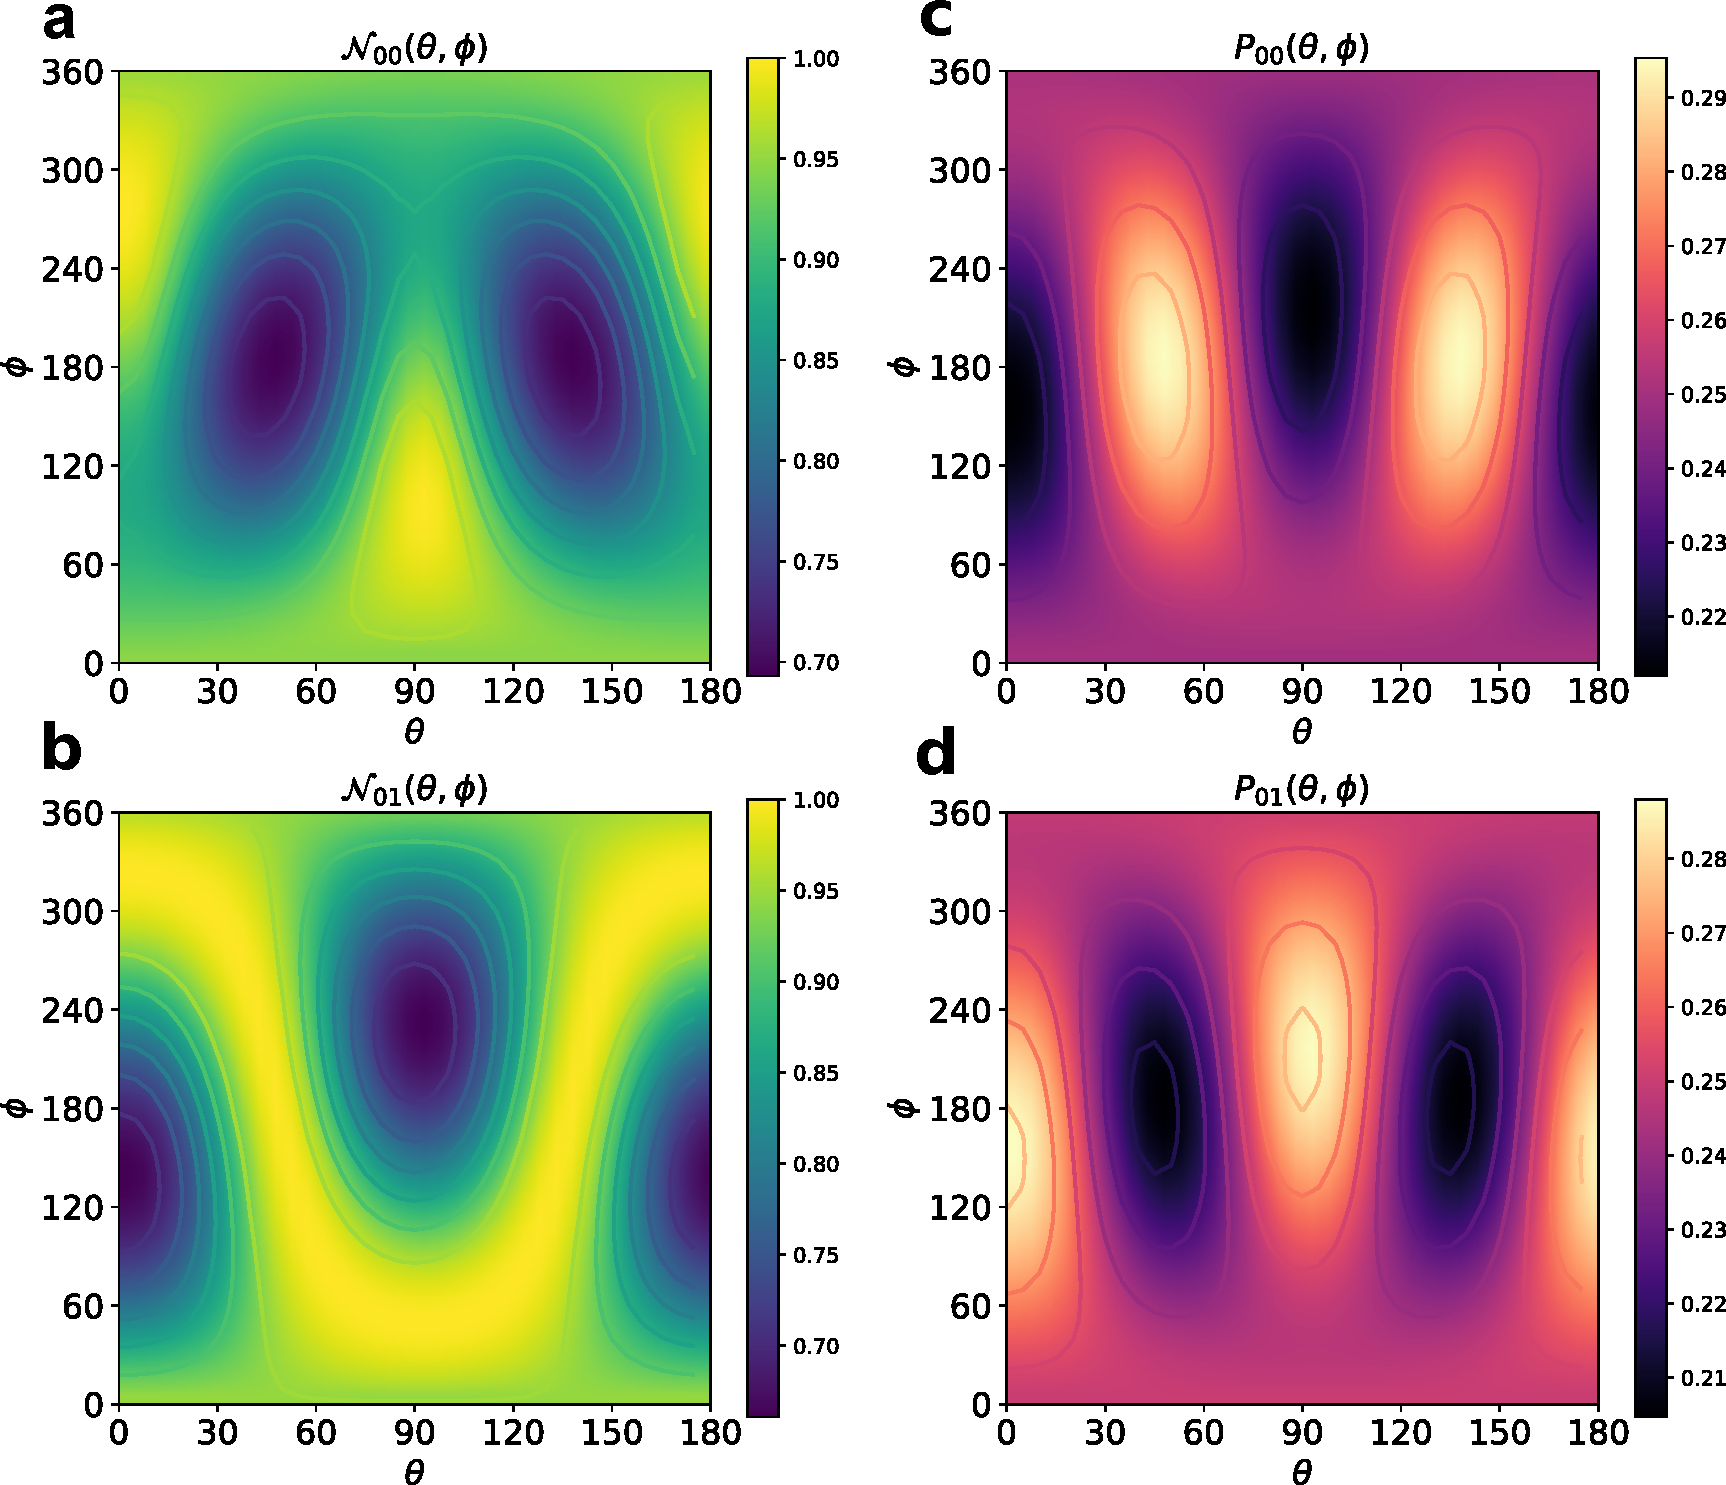
\includegraphics[width=\columnwidth]{NP10steps.pdf}
    \caption{\textbf{Entanglement transfer after coin projections (la devo rifare)} a-b) State log-negativities applying the projectors $\PP_{00}$ and $\PP_{01}$ (the other two cases display the same behaviour) in terms of $(\theta, \phi)$ that define the coin basis. In this simulation we consider two identical 10-step Hadamard QWs. c-d) Corresponding surface for the projection probabilities.}
    \label{fig:10steps_results}
\end{figure}
%This numerical investigation indicates that one can find the %projector on coin state, regardless the choice the unitary of %QW, for an optimal transfer of the ebit of entanglement to the %walker's spaces

\section{Entanglement accumulation}
\label{sec:entanglement_accumulation}

\parTitle{Section overview}
Here we investigate whether the entanglement transfer procedure can be applied iteratively, accumulating more and more entanglement into the state of the walkers' degrees of freedom.
For this purpose, after each successful entanglement transfer stage, which produces a state of the form
\begin{equation}
	(\ket{\gamma_1}\otimes\ket{\gamma_2})_{\calC}\otimes \ket{\Psi}_{\calW},
\end{equation}
we apply an operation restoring the entanglement between the coins, thus producing a state of the form
% \begin{equation}
	$\ket{\Psi}_{\calW}\otimes\ket{\Phi}_{\calC}$,
% \end{equation}
with $\ket{\Phi}\in\HC^{(1)}\otimes\HC^{(2)}$ some entangled state --- usually a maximally entangled one.
The QW evolution is then used to correlate each coin and walker degree of freedom locally, in order to make transfering the entanglement via local projections possible.

\parTitle{Output of single round of entanglement transfer}
Suppose one round of entanglement transfer was executed successfully.
We therefore have entanglement in the bipartition $\HW^{(1)}\otimes\HW^{(2)}$, while the coin spaces are separated.
Can we perform another round of QW evolutions to transfer even more entanglement to the walkers?

\parTitle{Entanglement accumulation, problem statement}
Let us consider, as an example, the case where $\ket{\Psi}_\calW$ has entanglement dimension $2$, and the full state has the form
\begin{equation}
	 \ket{\Psi} =
	\ket{\uparrow\uparrow}_{\calC}
	\otimes
	(\ket{\psi_1\psi_2} + \ket{\psi_2\psi_1})_{\calW}/\sqrt2,
\end{equation}
for some walker states $\ket{\psi_i}$ with $\braket{\psi_i}{\psi_j}=\delta_{ij}$.
% Note that we are assuming here for simplicity that the coins have been projected onto $\ket\uparrow$, and that the post-selected walker states form a singlet.
% While this is not generally the case, we can always formally describe the states this way, up to some relabelling \commale{for the coin part I agree (in fact, I guess it does not matter at all), for the walker part, this is an assumption, which however is based on the fact that analytically for 1-step/1-projection is true as proven analytically, am I right?}. 
Restoring the entanglement between the coins we get
\begin{equation}
	\ket{\Psi'} =
	(\ket{\uparrow\uparrow}+ \ket{\downarrow\downarrow})_{\calC}
	\otimes
	(\ket{\psi_1\psi_2} + \ket{\psi_2\psi_1})_{\calW}/2.
	\label{eq:ent_acc_initial_state}
\end{equation}
Let us, as in~\cref{sec:entanglement_transfer_local_projections}, focus on the transferability on $\calH^{(1)}$.
The reduced state $\rho^{(1)}\equiv\tr_2\PP_{\Psi'}$ has the form
\begin{equation}
	\rho^{(1)} =
	(\PP_\uparrow + \PP_\downarrow)_\calC
	\otimes
	(\PP_{\psi_1} + \PP_{\psi_2})_\calW/4.
\end{equation}
A QW evolution $\calW_{\calS}$ then gives
%\begin{equation}
%\begin{gathered}
$\PP[\calW_{\calS}\ket{\uparrow,\psi_1}] + 
	\PP[\calW_{\calS}\ket{\uparrow,\psi_2}] + 
	\PP[\calW_{\calS}\ket{\downarrow,\psi_1}] + 
	\PP[\calW_{\calS}\ket{\downarrow,\psi_2}]= \PP_{\Psi_1} + \PP_{\Psi_2} + \PP_{\Psi_3} + \PP_{\Psi_4}$,
%\end{gathered}
%\label{eq:accum}
%\end{equation}
where $\braket{\Psi_i}{\Psi_j}=\delta_{ij}$, and thus $\calW_{\calS}\rho^{(1)}\calW_{\calS}^\dagger$ has rank $4$.
Achieving entanglement transfer now entails finding a state $\ket\gamma$ such that
\begin{equation}
	\|\mel{\Psi_i}{\PP_\gamma\otimes I_\calW}{\Psi_j}\|^2 = \delta_{ij} p_{\on{proj}}.
\end{equation}
Each successive entanglement transfer iteration involves a doubling of the number of orthogonal states to preserve as follows from observing that if $A$ has rank $r$ and $B$ has rank $r'$, then $A\otimes B$ has rank $rr'$.
% More generally, given an reduced state $\rho^{(1)}\in\calH^{(1)}$ that is a mixture of orthogonal projectors, $\rho^{(1)}\simeq\sum_i\PP_{\psi_i}$,
% to achieve $\on{TC}_1$ after evolution through a unitary $\calU$ we need
% $\mel{\gamma}{\calU}{\psi_i}$ to be orthogonal with each other, that is,
% \begin{equation}
% 	\mel{\psi_i}{\calU^\dagger(\PP_\gamma\otimes I_\calW)\calU}{\psi_j} = p \delta_{ij}.
% \end{equation}

\parTitle{QWs with $C=I$}
Consider now a QW in which each coin operation is the identity: $\calC=I$.
We will show that, with this particular type of dynamics, we can accumulate arbitrary amounts of entanglement into the walkers' degrees of freedom, using the coins as mediators.
The unitary evolution corresponding to $n$ steps with $\calC=I$ is $\calW_{\calS n}=\calS^n$ with $\calS$ the controlled-shift operation.
The action on the basis states is then
\begin{equation}
    \calS^n = \PP_\uparrow \otimes I + \PP_\downarrow\otimes \EE_+^n,
\end{equation}
where $\EE_+\equiv \sum_k\ketbra{k+1}{k}$ is the operation shifting the walker's position, and $\EE_+^n$ is thus the operator moving the walker $n$ positions forward.
Consider an initial state
\begin{equation}
    (\ket{\uparrow,\uparrow}+\ket{\downarrow,\downarrow})_\calC\otimes
    \ket{\Psi}_\calW
    % \frac{1}{\sqrt r}\sum_{k=1}^r \ket{k,k}_{\calW},
\end{equation}
with $\ket{\Psi}_\calW$ and entangled state of the walkers in which the different between the final and initial occupied positions is $\ell\in\NN$
(for example, if $\sqrt2\ket{\Psi}_\calW=\ket{1,1}+\ket{3,3}$, then $\ell=2$).
If $\ket{\Psi}_\calW$ has rank $r$, the reduced state on $\calH^{(1)}$ has the form
\begin{equation}
    \tr_2(\PP_{\Psi}) = \frac12 (\PP_\uparrow+\PP_\downarrow)\otimes\sum_{k=1}^r p_k \PP_{\psi_k}
\end{equation}
for some set of orthonormal states $\{\ket{\psi_k}\}_k\subset\HW^{(1)}$.
Evolving through $\calS^{\ell+1}$, we get
\begin{equation}
    \tr_2(\PP_{\Psi}) \to
    \PP_\uparrow\otimes\sum_{k=1}^r p_k \PP_{\psi_k} +
    \PP_\downarrow\otimes\sum_{k=1}^r p_k \PP_{\psi_k'}
\end{equation}
with $\braket{\psi_j'}{\psi_k'}=\delta_{jk}$ and $\braket{\psi_j'}{\psi_k}=0$.
Then, any balanced projection $\ket\gamma=\frac{1}{\sqrt2}(\ket0+e^{i\phi}\ket1)$ achieves $\on{TC}_1$, which means that the entanglement can be transferred deterministically from coins to walkers. 

\parTitle{Specific optimal accumulation protocol}
In light of these findings, we can now propose the following explicit protocol, which allows to accumulate deterministically entanglement into the walkers degrees of freedom using the coins as mediators.
Starting from the state
$(\ket{\uparrow,\uparrow}+\ket{\downarrow,\downarrow})/\sqrt2\otimes\ket{1,1}\in\calH$,
we apply the conditional shift operation tow both QWs and then measure both coins in the basis $\ket\pm$. %=\frac{1}{\sqrt2}(\ket\uparrow\pm\ket\downarrow)$.
The possible states after the projection are then
%\begin{equation}
   $(\ket{1,1} \pm \ket{2,2})/\sqrt2$,
%\end{equation}
where the sign is $+$ if the two coins are found in the same state, and $-$ otherwise.
Restoring the entanglement between the coins, we then re-apply the QW evolution and project again in the basis $\ket\pm$, resulting in an output state of the form
\begin{equation}
    \frac12[(\ket{1,1}\pm\ket{2,2}) \pm (\ket{3,3} \pm \ket{4,4})].
\end{equation}
This procedure can be iterated to accumulate more and more entanglement in $\HW^{(1)}\otimes\HW^{(2)}$.
At the $n$-th iteration, we evolve both spaces through $2^n$ QW steps with $\calC=I$, that is, through the unitary $\calS^{2^n}\otimes\calS^{2^n}$, and then project onto the $\ket\pm$ basis,
resulting in a maximally entangled state of the form
\begin{equation}
    2^{-n/2}\sum_{k=1}^{2^n} (-)^{\sigma_k}\ket{k,k},
\end{equation}
with $(-)^{\sigma_k}\in\{1,-1\}$ for all $k$.

% This is a state in which there is an ebit of entanglement stored in the coin degrees of freedom, and $r$-dimensional entanglement stored between the positions.
% Evolving this state through $r$ steps of a QW with $C=I$, we obtain
% \begin{equation}
%     \ket{\uparrow,\uparrow}\otimes\left(
%         \sum_{k=1}^r \ket{k, k}
%     \right) +
%     \ket{\downarrow,\downarrow}\otimes\left(
%         \sum_{k=r+1}^{2r} \ket{k,k}
%     \right).
% \end{equation}
% Projecting both coins onto $\ket{\gamma_\phi}=\frac{1}{\sqrt2}(\ket0+e^{i\phi}\ket1)$, $\phi\in\RR$, thus produces a maximally entangled state in $\HW^{(1)}\otimes\HW^{(2)}$, with entanglement dimension $2r$, thus fully transferring the entanglement from $\HC^{(1)}\otimes\HC^{(2)}$ to $\HW^{(1)}\otimes\HW^{(2)}$.
% The probability of any such projection is $p_{\on{proj}}=1/2$.
% However, thanks to the freedom in the choice of $\phi$, both $\ket{\gamma_\phi}$ and $\ket{\gamma_{\phi+\pi}}$ are suitable projections, which implies that, measuring the polarization in any such measurement basis, the entanglement is optimally transferred regardless of the observed outcome, thus making the protocol deterministic.

% \parTitle{Explicit calculation QWs}
% Let us consider the case in which for simplicity the first projection is 00 type and the unitaries are identical. The input state for the second iteration, after the $U^{Bell}$ on the coin
% \begin{align}
%      \ket{\Psi^{0 (1)}} &= \frac{1}{2}\left(\ket{\uparrow \psi_a}_1 \ket{\uparrow \psi_b}_2 +\ket{\uparrow \psi_b}_1 \ket{\uparrow \psi_a}_2 + \right. \notag\\
%       &\left. + \ket{\downarrow \psi_a}_1 \ket{\downarrow \psi_b}_2 +
%      \ket{\downarrow \psi_b}_1 \ket{\downarrow \psi_a}_2
%      \right),
% \end{align}
% injected to the others QWs, will produce the state
% \begin{align}
%      \ket{\Psi^{f(1)}} &=
%      \alpha \ket{\Psi^{\uparrow \psi_a}_1\Psi^{\uparrow \psi_b}_2} +
%      \beta \ket{\Psi^{\uparrow \psi_b}_1\Psi^{\uparrow \psi_a}_2} +  \notag \\
%         &+ \delta \ket{\Psi^{\downarrow \psi_a}_1\Psi^{\downarrow \psi_b}_2} 
%          + \gamma \ket{\Psi^{\downarrow \psi_b}_1\Psi^{\downarrow \psi_a}_2}.
% \label{eq:final_state1}                 
% \end{align}
% It is clear \highlight{(is it?)} that after a further coin projection, the whole state will collapse in a superposition of four terms with at least four different qudits states involved.
% Due to the high-dimension of the two walkers position, we can generate states in which the four qudits in the superposition are mutually orthogonal.


% \parTitle{Scaling of negativity}
% The negativity of a maximally entangled state in $N$ dimensions, $\sum_{k=1}^N \ket{k,k}$, equals $\calN = \log_2(N+1)$.
% % Consider a state $\ket{q} = \frac{1}{\sqrt{n_q}}\sum_{s =1}^{n_q} \ket{ss}$, where $\ket{s}$ are a set of orthornormal states for the two-walker space.
% % The negativity of such state scales with respect to the dimension $n_q$ as $\log_2(n_q + 1)$.
% According to such intuition we expect that the maximum negativity of the output state of QWs after $N_i$ iterations of entanglement transfer via proper coin projection, could be $\mathcal{N}^{Max} =\log_2( 2^{N_i-1}+1)$.
% In ideal entanglement transfer conditions, iterating the entanglement transfer protocol $m$ times, we should therefore expect a final negativity of $\log_2(2^{m})=m$
% In such condition the number of orthogonal states in the output grows as $2^{N_i-1}$. This can be verified by comparing the state in \eqref{eq:qudit_ent} after one iteration, and the state after two iterations in eq.~\eqref{eq:accum}.

\parTitle{Numerical results \label{transfer}}
\LI{again, these numerics might be a bit obsolete at this point, or otherwise we should find a reason why we might need some numerics}
In~\cref{fig:entanglement_accumulation_numerical_results}a we report numerical results on the scaling of the negativity for different numbers of iterations.
We consider consecutive iterations with Hadamard QWs of equal steps $N$, and coin projection followed by a Bell-state generation in between. The input state is the one in~\cref{eq:ent_acc_initial_state}, with the entanglement between the two coins.
At each iteration the coin projection parameters are optimized to obtain a state with the highest negativity, using the projectors of type $\PP_{00}$ (see section \ref{transfer})
We find that in this condition the optimal curve $\mathcal{N}^{Max}$ is not saturated, in which we expect to accumulate one-ebit per iteration. This result thus confirms that to saturate this bound we need to chose accurately the coin projection, as in the case of one iteration, and the QWs routines of the subsequent iterations.
% Different strategies can be investigated to improve the performance of the protocol.
In the histograms in~\cref{fig:entanglement_accumulation_numerical_results}b we report the distributions of the state negativity after two iterations of entanglement transfer. In the first iteration the QWs are identical with Hadamard coins. For the next iteration we sample 500 coin operators to be applied at each step of the two local QWs.
It is possible to find QW unitaries that saturates the maximum state negativity for two iteration set to 2. Furthermore it seems easier to find this unitaries by considering higher number of steps (see~\cref{fig:entanglement_accumulation_numerical_results}b). The latter result is not surprising, since with many steps we cover higher-dimensional Hilbert spaces and, consequently, it is easier to produce four mutually orthogonal qudits.

\commale{would it be possible to go beyond 2 iterations, optimizing the QW unitary, to get the maximal entanglement accumulation?}



\begin{figure}[tb]
	\centering
    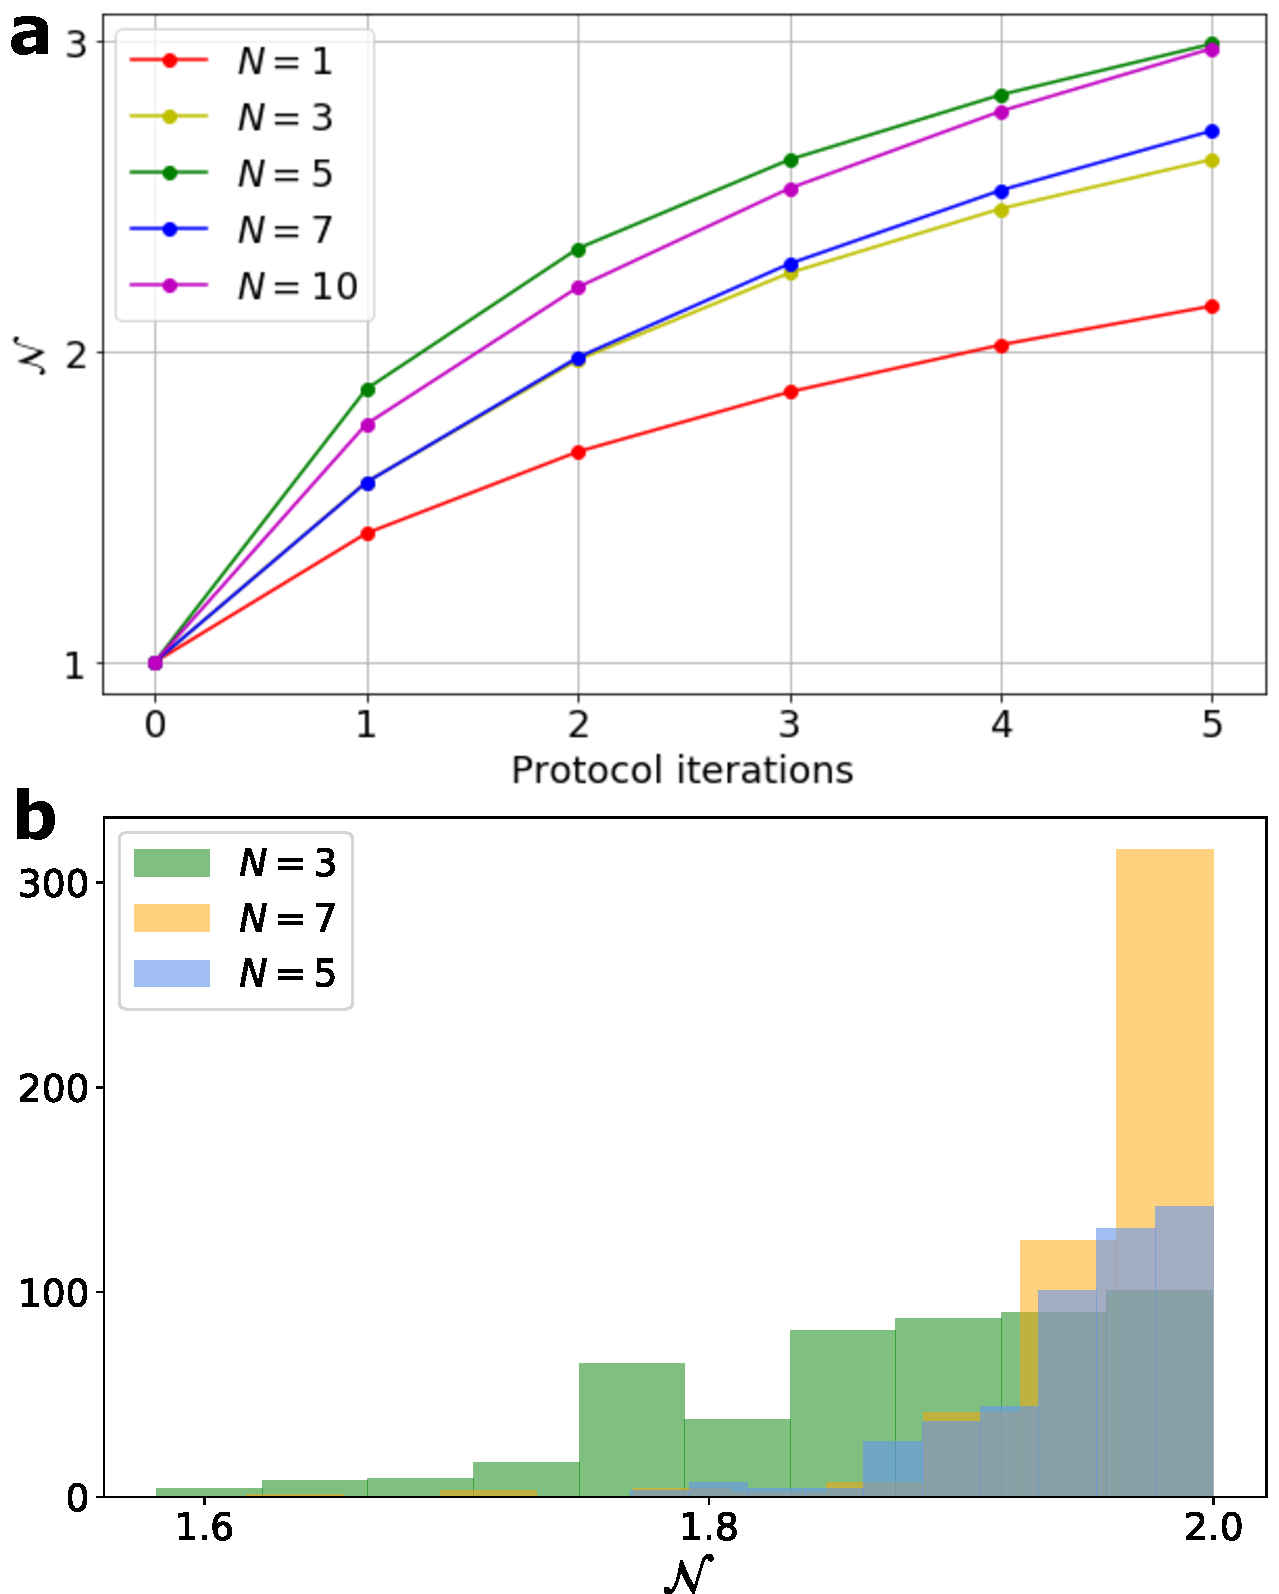
\includegraphics[width = \columnwidth]{figures/entanglement_accumulation_results.pdf}
    \caption{\textbf{Entanglement accumulation}
    \textbf{a)} Negativity for different iterations of the entanglement transfer protocol. Both parties evolve according to identical Hadamard QWs, for $N=1,3,5,7,10$ steps. From such simulation seems that the optimal transfer of one ebit per iteration cannot be reached. However, allowing for different unitaries at each iteration, the optimal scaling is recovered.
    \LI{maybe redo figure using $2^n$ steps for $n$ iterations.}
    \textbf{b)} Histograms for two iterations of entanglement transfer protocol (the first with two identical Hadamard QWs), for $N=3,5, 7$ QW steps \LI{why not both random?}. 
    Each histograms represent the distribution of $500$ random extracted coin operators \LI{are the coin ops randomly sampled at each step, or does each tested QW use the same coin op at all steps?} for individuating the QW unitary to apply to the two walkers in the state $\ket{\Psi^{0(1)}}$. We observe that it is possible to find unitary operations for the second entanglement transfer which allows to saturate the bound of 2 ebit of entanglement. In particular histograms tend to pick towards 2 with increasing number of steps. All the calculations were performed considering coin projection of type $\PP_{00}$.
    \LI{potrebbe essere utile avere evidenza numerica per step}
    \LI{the labels in the legend are out of order}
    }
    \label{fig:entanglement_accumulation_numerical_results}
\end{figure}


\section{Entanglement retrieval}
\label{sec:entanglement_retrieval}

The arguments of~\cref{sec:entanglement_transfer_local_projections} do not make assumptions on the dimensions of $\HC^{(i)}$ and $\HW^{(i)}$. This means that they can be used not only to study the transfer of entanglement from coins to positions, but also the other way around.
For example, if the initial reduced state on $\calH^{(1)}$ is
%\begin{equation}
    $[\PP_\uparrow\otimes (\PP_1+\PP_2)]/2$,
%\end{equation}
with $\ket1,\ket2$ a pair of orthonormal walker's states, then applying an Hadamard operation to the coin, and two steps of QW evolution with $\calC=I$, we obtain the state
\begin{equation}
    \frac14[\PP_\uparrow\otimes(\PP_1+\PP_2) + \PP_\downarrow\otimes(\PP_3+\PP_4)].
\end{equation}
Then, measuring in the Hadamard four-dimensional basis --- \textit{i.e.}, the basis formed by the columns of the $4\times4$ Hadamard matrix --- we achieve $\on{TC}_1$.

% Let us investigate the inverse process for the entanglement transfer, namely from the the state of two entangled walkers to the space of the two coins. Here the question is if it is always possible to saturate the maximal amount of entanglement transferable to the space of two qubits. In other word if we can obtain a Bell-like state with one ebit of entanglement via two local identical quantum walks routines and a suitable single-qudit projection in the walker subspace. 

% Let's start from the simplest case, an initial state as
% \begin{equation}
%     \ket{\Psi_0}=\frac{1}{\sqrt{2}}\ket{\uparrow\uparrow}\otimes
%     ( \ket{\psi_a\psi_a}+\ket{\psi_b\psi_b})
% \end{equation}
% in which we require $\braket{\psi_a}{\psi_b}=0$, in order to have one ebit of entanglement at the beginning of the process. Furthermore the dimension $d_0$ of each walkers subsystem is at least two, $d_0\geq 2$. Under the hypothesis of the evolution according to two identical local QWs routine, the final state becomes
% \begin{equation}
%     \ket{\Psi_f}=\frac{1}{\sqrt{2}}(\ket{\Psi^{\uparrow a}\Psi^{\uparrow a}}+\ket{\Psi^{\uparrow b}\Psi^{\uparrow b}})
%     \label{eq:retr1}
% \end{equation}
% According to the notation of the previous sections, the states $\ket{\Psi^{\uparrow i}}$ are the output of a single-particle QW given as input the coin state $\ket{\uparrow}$ and the walker in $\ket{\psi_i}$. Given the structure of QW's evolution that correlates the two degree of freedoms, the coin and the positions, we can express the $\ket{\Psi^{\uparrow i}}$ as
% \begin{align}
%     \ket{\Psi^{\uparrow a}}&= a_0\,\ket{0\,\phi_{a_0}} +a_1\,\ket{1\,\phi_{a_1}} \notag\\
%     \ket{\Psi^{\uparrow b}}&= b_0\,\ket{0\,\phi_{b_0}} +b_1\,\ket{1\,\phi_{b_1}}
%     \label{eq:retr2}
% \end{align}
% where $\{\ket{0},\ket{1}\}$ is a generic orthonormal basis for the coin subspace and the $\ket{\phi_{i_j}}$ the projections of the state $\ket{\Psi^{\uparrow i}}$ in this basis. 
% Now we look for the local qudit projector $\hat{P}_{\phi}=\ketbra{\phi}$ acting on the single subsystem for obtaining a Bell-like state in the two coins. Let us label the overlaps between $\phi$ and single qudit states $\ket{\phi_{i_j}}$ in \eqref{eq:retr2} as
% \begin{equation}
%     \braket{\phi}{\phi_{i_j}}=\beta_{ij}
% \end{equation}
% where we remind that index $i=\{a,b\}$ and $j=\{0,1\}$. Then the state after the projection $\hat{P}_{\phi}$ in the two subsystems
% \begin{equation}
% \begin{split}
%     \braket{\phi}{\Psi_f}&=\frac{1}{\sqrt{2}}[(a_0a_1\beta_{a0}\beta_{a1}
%     + b_0b_1 \beta_{b0}\beta_{b1})(\ket{01}+\ket{10})+\\
%     &+(a_0^2\beta_{a0}^2+b_0^2\beta_{b0}^2)\ket{00}+ (a_1^2\beta_{a1}^2+b_1^2\beta_{b1}^2)\ket{11}]
% \end{split}
% \end{equation}
% Let us observe that a Bell-like state in the form $\frac{1}{\sqrt{2}}(\ket{00}+\ket{11})$ can be retrieved by requiring for example that 
% \begin{align}
% \beta_{a0}&=\beta_{b1}=0 \label{eq:retr_cond1}\\
% \frac{\beta_{a1}}{\beta_{b_0}}&= e^{i \alpha} \frac{b_0}{a_1} \label{eq:retr_cond2}
% \end{align}
% [da scrivere il caso generale con n-ebit in ingresso]



% \section{Purity of reduced states}
% \label{sec:purity_reduced_states}

% \begin{figure*}[t]
%     \centering
%     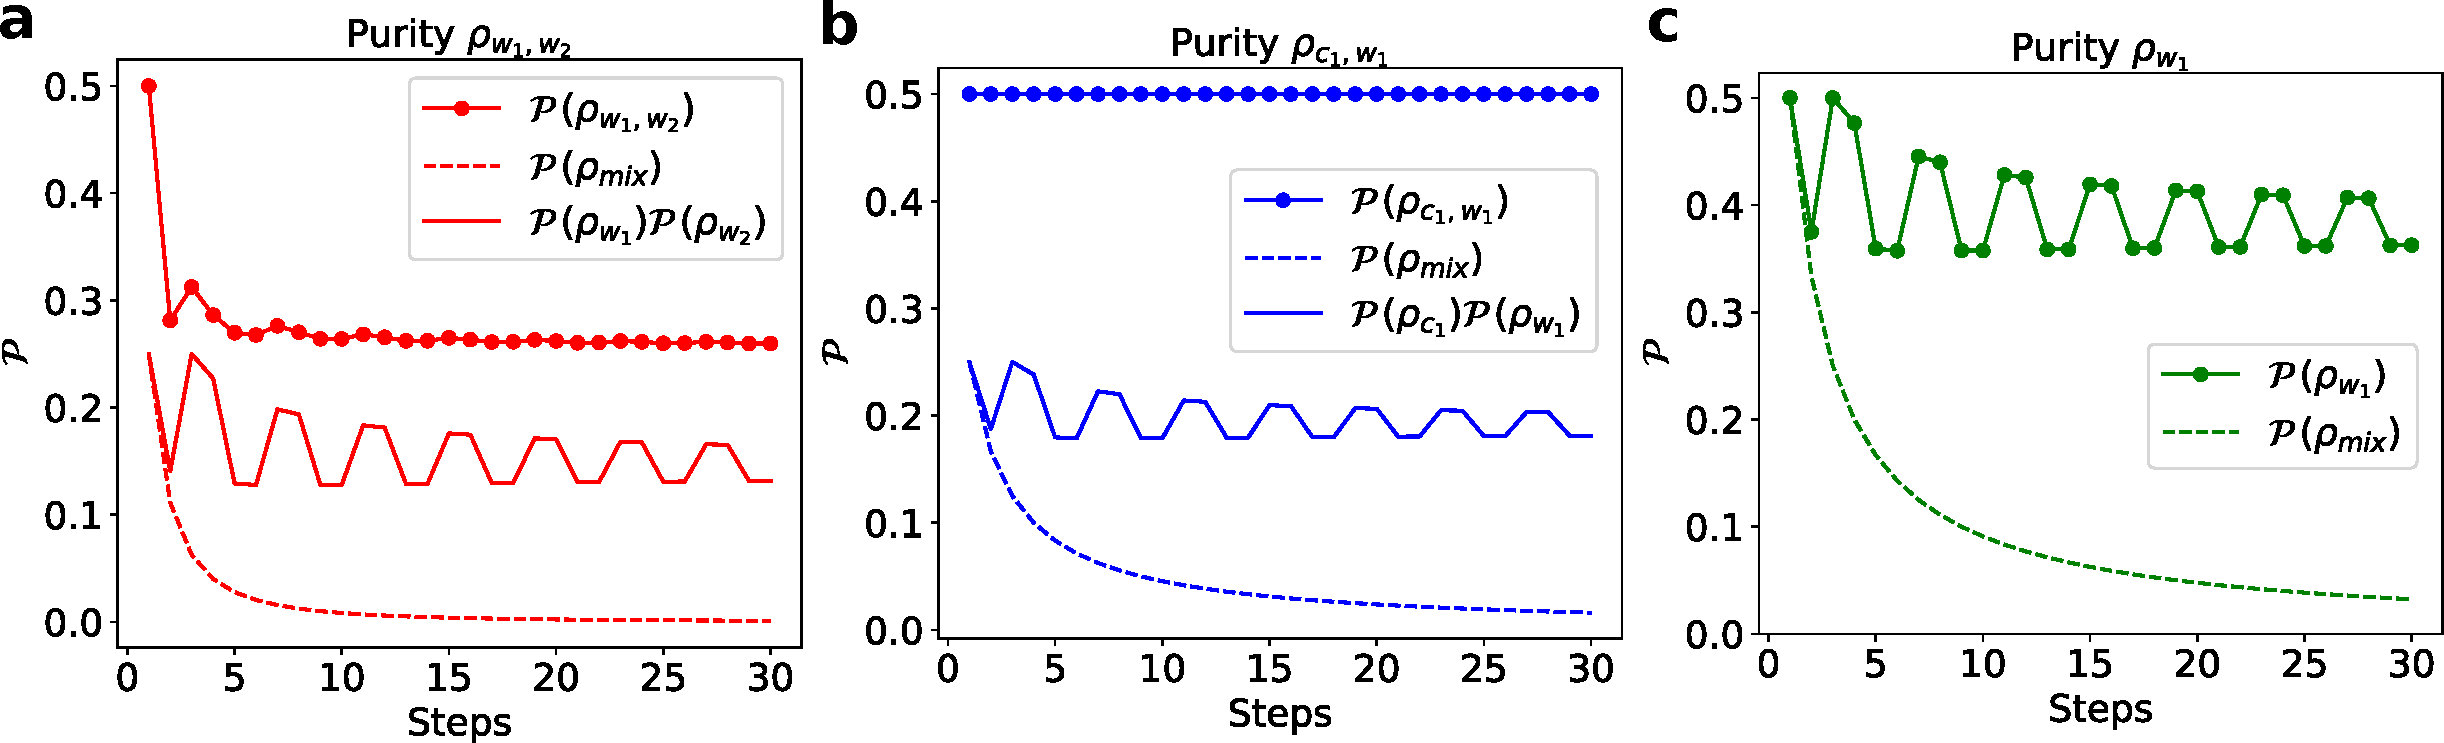
\includegraphics[width=\textwidth]{purity_of_reduced_states.pdf}
%     \caption{\textbf{Purity of traced subsystems}.
%     In each panel we report the purity of the state for different number of steps, of two identical Hadamard quantum walks. The dashed line correspond to the purities of the classical statistical mixture associated to the subspace after investigation.
%     \highlight{(I don't understand what $\rho_{\on{mix}}$ represents. It should also probably be mentioned in the text.)}\\
%     \highlight{(Mention why we include the product of purities as well.)}\\
%     \highlight{(why do only the upper lines use dots? I would add dots (or other marker) on all lines (or none))}\\
%     \highlight{(comment on the peculiar zigzagging behaviours)}
%     }
%     \label{fig:purity_traced_subsystems}
% \end{figure*}

% \parTitle{Why do we do this?}
% The state purity of the traced subsystem could provide a first insight on the entanglement structure of the state. \highlight{(we should probably justify this a bit more)}

% \parTitle{What exactly are we computing}
% We study here the purity of reduced states at different stages of a Hadamard QW evolution \highlight{(define what this is (if not done before), and comment why we use \textit{Hadamard} QW)}.
% More specifically, we consider the purities of
% \begin{enumerate}
%     \item the walkers' states $\rho_{w_1,w_2}=\tr_{c_1,c_2}(\rho)$,
%     \item a single particle's state: $\rho_{w_1,c_1}\equiv\tr_{c_2,w_2}(\rho)$,
%     \item a single walker's state $\rho_{w_1}\equiv\tr_{c_1,w_2,c_2}(\rho)$.
% \end{enumerate}
% Each quantity is computed on the outputs of the Hadamard QW after different numbers of steps, as reported in~\cref{fig:purity_traced_subsystems}
% \highlight{(justify why these particular choices (e.g. why not also $\rho_{c_1}$?)}
% If $\rho_{w_1,w_2}=\rho_{w_1}\otimes\rho_{w_2}$, then $\mathcal{P}(\rho_{w_1,w_2}) = \mathcal{P}(\rho_{w_1}) \mathcal{P}(\rho_{w_2})$, where $\calP(\rho)\equiv\tr(\rho^2)$ denotes the purity of the state.
% In~\cref{fig:purity_traced_subsystems}a we show that $\calP(\rho_{w_1,w_2})>\calP(\rho_{w_1})\calP(\rho_{w_2})$, and similarly for $\rho_{c_1,w_1}$,
% revealing the presence of residual correlations between walkers, and between the internal degrees of freedom of the individual particles \highlight{(these can be purely classical correlations though. The purity not being factorisable only rules out product states, not separable ones. Consider \textit{e.g.} $(\ketbra{00}+\ketbra{11})/2$)}.
% This is further confirmed by the negativities reported in~\cref{fig:neg_trace}a.


% \parTitle{Results for general case}
% We then consider the most general cases, namely two different unitaries transformation made by random step-dependent coin operators. In~\cref{fig:neg_trace}b and c we report the histograms for the negativities of $\rho_{w_1,w_2}$ and $\rho_{c_1, w_1}$, computed on samples of $1000$ pairs of random unitaries $(U_1,U_2)$ \highlight{(how were these sampled? uniformly random or something else?)}, for different step numbers. The histograms seem to become more peaked around higher values of negativities with increasing numbers of steps \highlight{(meaning...?)}.

% \parTitle{What did we conclude from this?}

% \begin{figure*}[hbt]
%     \centering
%     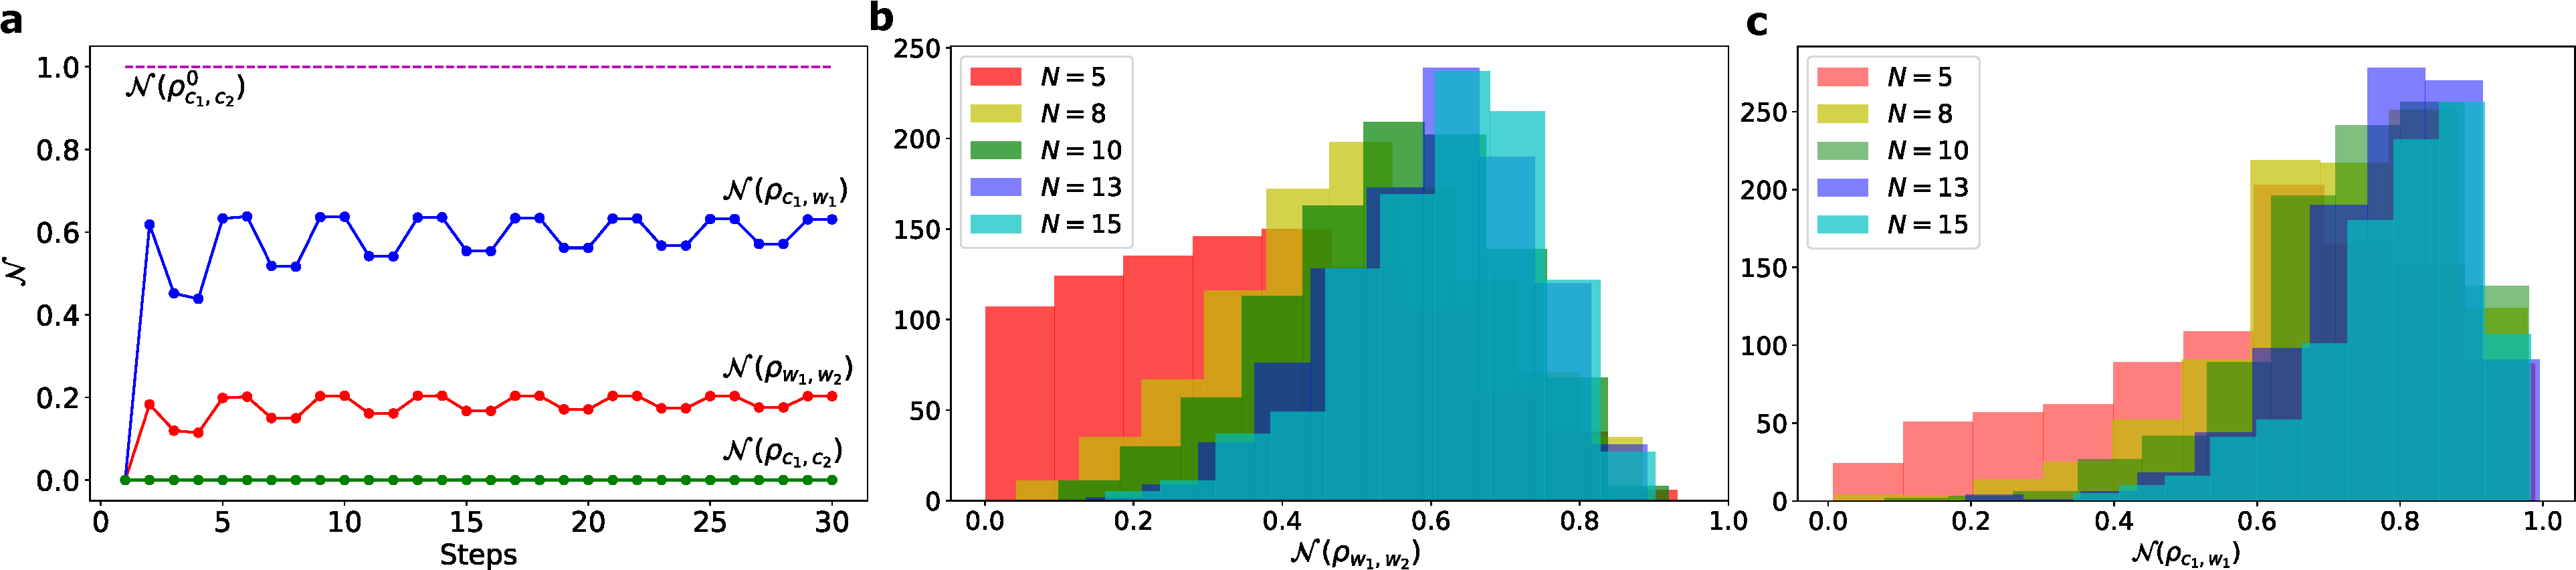
\includegraphics[width=\textwidth]{figures/negativity_histograms.pdf}
%     \caption{\textbf{Negativity criterion}.
%     (a) Negativity, at each step of the Hadamard QWs, of different reduced states.
%     % We consider in red the subsystems associated to the two walkers positions $(w_1,w_2) $ tracing the two coin, in green the system of the two coin tracing the positions $(c_1, c_2)$ and in blue the system of a single quantum walker tracing the other one, namely $(c_1, w_1)$ in the plot.
%     In magenta (dashed line) we report for reference the negativity of the initial Bell state in the coin degree of freedom.
%     We observe a non-zero negativity between the two walkers. (b-c) Negativities of $\rho_{w_1, w_2}$ and $\rho_{c_1, w_1}$ computed for $1000$ random unitaries. Relaxing the condition of identical QWs and allowing the coin to change at each step, higher values of negativities can be obtained. Furthermore the average increases with the number of step.}
%     \label{fig:neg_trace}
% \end{figure*}



\section{Experimental proposal}
\label{sec:experimental_proposal}
Here we propose a scheme for the realization of the entanglement accumulation protocol in a photonic platform that encodes coin and walkers position in polarization and OAM degree of freedom. This proposal provides the realization of two iterations, giving access to states with 2 ebit of entanglement. 

The scheme requires that, at the first iteration, the two QWs are identical and we perform type-00 projections on the coins \textcolor{blue}{MP: dovremmo spiegare che significa type 00?}. In this way, the state after the projection that maximize the negativity will be $\ket{\uparrow \uparrow}\otimes(\ket{\psi_a\psi_b}\pm\ket{\psi_b\psi_a})/\sqrt2$. 
It is straightforward to show that the action of a polarizing beam-splitter combined with two half-waveplates can perform, with probability $1/2$, the transformation needed to achieve accumulation, resulting in the output state
%Indeed, rewriting the state in terms of creation operators we have:
%\begin{equation}
  %  \frac{1}{\sqrt{2}}\left(a^{\dagger}_{\uparrow, \psi_a,1}a^{\dagger}_{\uparrow, \psi_b,2}+a^{\dagger}_{\uparrow, \psi_b,1}a^{\dagger}_{\uparrow, \psi_a,2} \right)\ket{0} 
    %\label{eq: snd_quant}
%\end{equation}
%The two photon are injected in the two input port of a polarizing beam-splitter, after a polarization rotation made by two half-waveplates (see~\cref{fig:conceptual_fig_2}). Then creator operators in \cref{eq: snd_quant} become

%\begin{equation}\begin{aligned}
%    a^{\dagger}_{\uparrow, \psi_{a/b},1} & \rightarrow \cos{\theta_1}a^{\dagger}_{\uparrow, \psi_{a/b},1} + i\sin{\theta_1}a^{\dagger}_{\downarrow, \psi_{a/b},2} \\
 %   a^{\dagger}_{\uparrow, \psi_{a/b},2} & \rightarrow \cos{\theta_2}a^{\dagger}_{\uparrow, \psi_{a/b},2} + i\sin{\theta_2}a^{\dagger}_{\downarrow, \psi_{a/b},1}
%\end{aligned}\end{equation}

\begin{figure}[t]
    \centering
    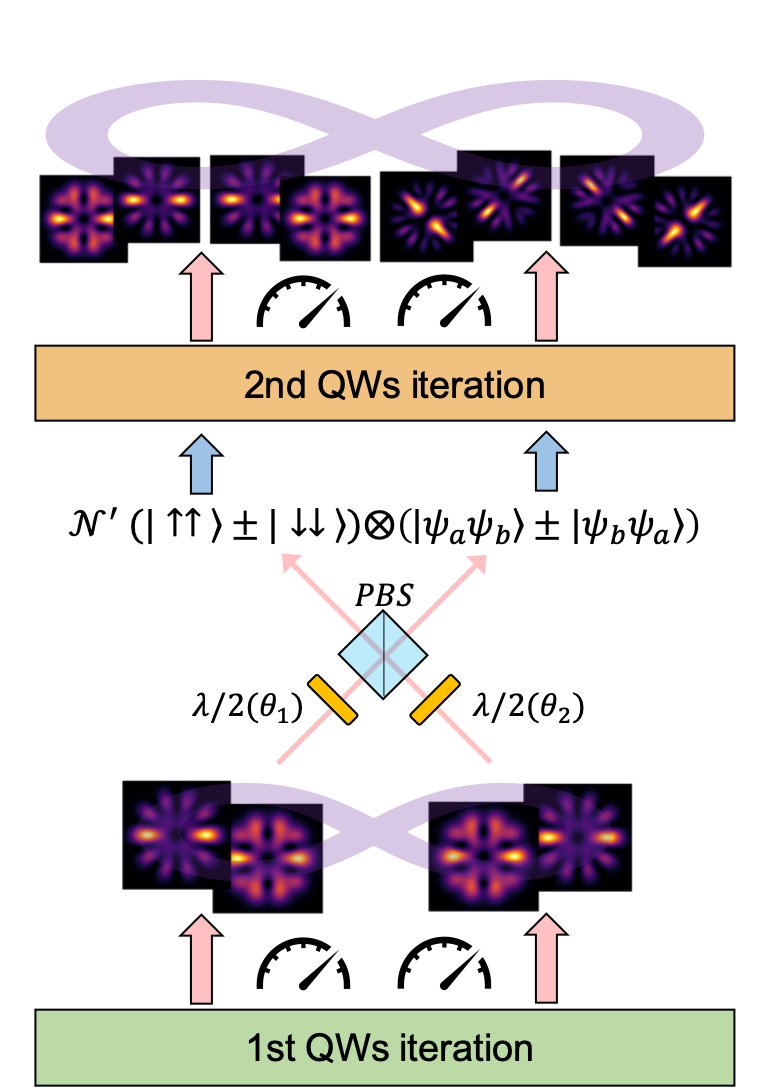
\includegraphics[scale= 0.45]{figures/conceptual_fig_2.png}
    \caption{\textbf{Experimental proposal}}
    \label{fig:conceptual_fig_2}
\end{figure}


%Substituting such expression in \cref{eq: snd_quant} and considering $\theta_1 = \theta_2$ we obtain 
\begin{align}
\frac{1}{2} \frac{\left( \ket{\uparrow \uparrow} \pm
\ket{\downarrow \downarrow}\right) }{\sqrt{2}}\otimes \frac{\left( \ket{\psi_a \psi_b} \mp
\ket{\psi_b \psi_a}\right) }{\sqrt{2}} +\frac{1}{2}\frac{\left( \ket{20} +
\ket{02}\right) }{\sqrt{2}}
\end{align}
The first part of this state embodies the resource needed for the protocol accumulation. We can discard the second contribution by post-selecting two-fold coincidences between single-photon detectors at the end of the second iteration. It is worth noting that the probabilistic generation of the second maximally entangled state is due by the choice to encode qubits in photons. However, we remark that we could also consider the state produced by the projection 11 after the first operation. Indeed it produces, with the same set of optimal $(\theta, \phi)$ parameters, states with the same symmetry properties. In this way it is possible to double the probability of generating states with more than one-ebit of entanglement.

%After a first research in literature, the maximum amount of entanglement generated with %OAM seems to be 3 ebit. In Ref. \cite{Malik2016}, the authors produce 3 entangled %qutrits in a 3-photon experiment.

\section{Conclusions}

We have addressed the generation of high-dimensional entangled states through a protocol of entanglement transfer from a low-dimensional resources. we have identified general transfer conditions that, if met, guarantee the successful pouring of any entanglement initially contained in the state of the resource to the high-dimensional {\it receiver}. This has then allowed us to draw a specific analysis aimed at the dynamics entailed by a QW, where low-dimensional resources and high-dimensional receivers are naturally embodied by coin and walker degrees of freedom. While characterizing the performance of the entanglement transfer scheme, we have been able to design schemes for entanglement accumulation and retrieval, thus drawing a complete picture for the manipulation of entanglement through a hetero-dimensional interface of great experimental potential. Indeed, the QW-based protocols addressed and studies in this paper are fully amenable to an implementation making use of polarization and OAM encoding. The scenario set by our schemes sets a promising framework for the use of low-dimensional entanglement as a resource to achieve otherwise complex entangled structures and states that can be experimentally synthesised and exploited. 


\begin{acknowledgments}

This work is supported by MIUR via PRIN 2017 (Progetto di Ricerca di Interesse Nazionale): project QUSHIP (2017SRNBRK), 387439. The authors acknowledge financial support from H2020 through the Collaborative Project TEQ (Grant Agreement No.  766900), the DfE-SFI Investigator Programme (Grant No. 15/IA/2864), the Leverhulme Trust Research Project Grant UltraQute (grant nr.~RGP-2018-266), COST Action CA15220, and the Royal Society Wolfson Research Fellowship scheme (RSWF\textbackslash R3\textbackslash183013).
\end{acknowledgments}

\appendix

% \section{Entanglement accumulation}

% \parTitle{The question}
% Can this type of entanglement transfer be performed multiple times?
% In other words, after a successful round of entanglement transfer, which results in a state of the form $\ket*{\psi_{AD}}\otimes\ket{\gamma_B\gamma_C}$
% with $\ket*\psi_{AD}$ (possibly maximally) entangled,
% can we apply the same procedure to transfer more entanglement into $\calH_{AD}$ by using $\calH_{BC}$ as medium?

% \parTitle{Why it is hard}
% The main hurdle in doing this is that the initial state is now of the form
% $\ket*{\psi_{AD}}\ket{\psi_{BC}}$ with \emph{$\ket*{\psi_{AD}}$ and $\ket*{\psi_{BC}}$ both entangled}.
% In the $n=2$ case, this amounts to the reduced state on $\calH_{AB}$ being a mixture of four orthogonal states, and one needs to find a projection $\ket\gamma$ which maintains their orthogonality.
% The problem with this type of procedure is that a local projection in $\calH_B$ amounts to a channel in $\calH_A$ which cannot sustain the orthogonality of more than $\dim(\calH_B)$ orthogonal states. From a more physical perspective, this means that such an operation cannot transfer more entanglement than the one that can fit in $\calH_B$.

% \parTitle{Example 1} Suppose the state after a successful round of entanglement transfer, and after a unitary has been applied to $\calH_{BC}$ to restore the entanglement, is
% \begin{equation}
%     \frac12 (\ket{HH} + \ket{VV})_{BC} \otimes (\ket{11} + \ket{22})_{AD}.
% \end{equation}
% Then applying twice a controlled-shift operation $\calS$, like the one used for discrete-time quantum walks: $\calS\ket{H,i}=\ket{H,i}$ and $\calS\ket{V,i}=\ket{V,i+1}$, we end up with a state which, reduced to $\calH_{AB}$, is spanned by the four orthogonal vectors
% \begin{equation}
%     \ket{H,1}, \,\,\ket{H,2}, \,\,\ket{V,3}, \,\,\ket{V,4}.
% \end{equation}
% % \begin{equation}
% % \begin{aligned}
% %     &\ket*{u^1} = \ket{H, 0}, \qquad
% %     \ket*{u^2} = \ket{H, 1}, \\
% %     &\ket*{u^3} = \ket{V, 2}, \qquad
% %     \ket*{u^4} = \ket{V, 3},
% % \end{aligned}
% % \end{equation}
% Projecting over $\ket{\gamma}_B$ is then easily seen to preserve the orthogonality of these four vectors, and therefore achieve entanglement transfer.
% The state after projecting over $\ket{\gamma}_B$ is then
% \begin{equation}
%     \frac12\left[
%         \ket{H}_C\otimes(\ket{11}+\ket{22}) +
%         \ket{V}_C\otimes(\ket{33} + \ket{44})
%     \right],
% \end{equation}
% and similarly projecting in $\calH_C$ we get the final state
% \begin{equation}
%     \frac12 (\ket{11} + \ket{22} + \ket{33} + \ket{44}) \in\calH_{AD}.
% \end{equation}

\section{Entanglement decreases if orthogonality is not preserved}
\label{proof1}
Let us show that if $\braket{\tilde u_j}{\tilde u_k}\neq\delta_{jk}$ then the Schmidt coefficients must change upon projection.
Indeed, in this case, $\ket{\Psi_\gamma}$ has the form
$\ket{\Psi_\gamma}=\sum_k \sqrt{\tilde p_k} \ket{\tilde u_k}\ket{v_k}$ where $\braket{v_j}{v_k}=\delta_{jk}$ and $\sum_k \tilde p_k=1$.
Denoting with $\Psi_\gamma$ the matrix whose vectorization is $\ket{\Psi_\gamma}$, this Schmidt decomposition amounts to the singular value decomposition $\Psi_\gamma = U\sqrt DV^\dagger$, with $D=\on{diag}(\tilde p_1,...,\tilde p_n)$, $V$ the unitary matrix whose columns are $\ket{v_k}$, and $U$  the (non-unitary) matrix with columns $\ket{\tilde u_k}$.
Then
\begin{equation}
    \Psi_\gamma\Psi_\gamma^\dagger = U D U^\dagger
    = \sum_k \tilde p_k \PP_{\tilde u_k},
\end{equation}
where $\PP_{\tilde u_k}=\ketbra{\tilde u_k}$ are in general non-orthogonal rank-$1$ projectors.
Let us then prove that if a matrix is a convex combination of rank-$1$ projections, then it always majorizes the vector of coefficients of the convex combination.
In our case, this translates to $\sum_k \tilde p_k\PP_{\tilde u_k}\succeq \tilde{\bs{p}}$.
% This allows us to conclude that, to transfer entanglement without degrading, it is necessary to find a projection $\ket\gamma$ that preserves the orthogonality of the states $\ket{u_k}$, and on top of this, the associated projection probabilities $\lvert\braket{\gamma}{u_k}\rvert^2$ must be equal to each other.

%\parTitle{Proof to possibly move to appendix or something}
Let $P_k$ be rank-$1$ projections, $p_k\ge0$ coefficients such that $\sum_{k=1}^n p_k=1$, and
$A\equiv \sum_{k=1}^n p_k P_k$. We want to prove that $A\succeq \bs p$,
% ~\footnote{Here, given $A$ Hermitian with $\tr(A)=1$ and $p_k\ge0$ with $\sum_k p_k=1$, we take $A\succeq\bs p$ to mean that the vector of eigenvalues of $A$, $\bs\sigma(A)$, majorizes the vector $\bs p$: $\bs\sigma(A)\succeq\bs p$.},
where $\bs p=(p_k)_{k=1}^n$ is the vector of coefficients, and the majorization relation is defined on Hermitian matrices via the corresponding vector of eigenvalues, that is,
$A\succeq\bs p\Longleftrightarrow \bs\sigma(A)\succeq\bs p$ where $\bs\sigma(A)$ is the vector of eigenvalues of $A$. If $A$ has dimension larger than $n$, we define $\bs\lambda(A)$ as the vector of the $n$ largest eigenvalues, in order to make the majorization relation well-defined.
Without loss of generality, let us assume that the $p_k$ are in decreasing order: $p_1 \ge p_2 \ge ...\ge p_n$.
Define the partial sums $A_\ell\equiv \sum_{k=1}^\ell p_k P_k$, so that $A=A_n$.
Observe that $A_\ell \ge A_r$ whenever $\ell\ge r$.
Because $\rank(P_k)=1$ for all $k$, we must also have $\rank(A_\ell)\le \ell$.
Denoting with $\lambda_j^\downarrow(A)$ the $j$-th largest eigenvalue of $A$, this implies that
\begin{equation}
    \sum_{k=1}^\ell \lambda_k^\downarrow(A_\ell) = \tr(A_\ell)
    = \sum_{k=1}^\ell p_k.
\end{equation}
Using $A=A_n\ge A_\ell$ for all $1\le \ell< n$, we thus conclude that
\begin{equation}
    \sum_{k=1}^\ell \lambda_k^\downarrow(A) \ge 
    \sum_{k=1}^\ell \lambda_k^\downarrow(A_\ell)
    = \sum_{k=1}^\ell p_k \equiv \sum_{k=1}^\ell p_k^\downarrow,
\end{equation}
that is, $\bs\lambda(A)\succeq \bs p$, which is the definition of $A\succeq \bs p$.

\parTitle{Entanglement degradation for different probabilities}
Assuming $\ket{\tilde u_k}$ are orthogonal, then the Schmidt coefficients of $\ket{\Psi_\gamma}$ are $\sqrt{\tilde p_k}=p^{-1/2}_{\on{proj}}\sqrt{p_k q_k}$.



\section{Proof of main result}
\label{appB}

Define $M\equiv \tr_{\calW}(\ketbra{u}{v})$, and notice that $\tr M=0$.
Assuming $M$ is diagonalizable and $M\ket{\lambda_\pm}=\pm\lambda\ket{\lambda_\pm}$, define
\begin{equation}
    \ket\gamma\equiv N\left(
        \ket{\lambda_+} +
        e^{i\arg\braket*{\lambda_-}{\lambda_+}} \ket{\lambda_-}
    \right),
    \label{eq:definition_projgamma_2dcase}
\end{equation}
where $N$ is a normalisation constant. Note that in general $\braket*{\lambda_+}{\lambda_-}\neq0$, as $M$ needs not be normal 
% \LI{prob move expr after general case}.
% A sufficient condition for $M$ to be diagonalizable is that $\det M\neq0$, which implies that
% $\{\braket*{H}{u^H},\braket*{V}{u^H}\}$ and
% $\{\braket*{H}{u^V},\braket*{V}{u^V}\}$
% are both linearly independent and nonzero \commale{I am lost in the notation here, have you defined $\ket{H}$ etc?}.

\parTitle{Proof for $M$ normal}
If $M$ is normal, then
\begin{equation}
	M = \lambda( \ketbra{v_1} - \ketbra{v_2}),
\end{equation}
for some $\lambda\in\CC$ and $\braket{v_i}{v_j}=\delta_{ij}$.
Then,
\begin{equation}
	\sqrt2\ket{\gamma_\phi} = \ket{v_1} + e^{i\phi}\ket{v_2}, \quad \phi\in\RR
\end{equation}
are suitable projections such that $\mel{\gamma_\phi}{M}{\gamma_\phi}=0$.
% The singular value decomposition of $M$ reads
% \begin{equation}
% 	M = s_1 \ketbra{v_1}{w_1} + s_2 \ketbra{v_2}{w_2},
% \end{equation}
% where $\braket{v_1}{v_2}=\braket{w_1}{w_2}=0$, $s_i\ge0$, and $\tr M=0$ translates into
% % \begin{equation}
% 	$s_1\braket{w_1}{v_1} + s_2 \braket{w_2}{v_2}=0$.
% % \end{equation}
% Consider the projections
% \begin{equation}
% \begin{aligned}
% 	\sqrt2\ket*{\gamma_\pm} &= \ket{w_1} \pm \ket{w_2}, \\
% 	\sqrt2\ket*{\gamma_\pm'} &= \ket{v_1} \pm \ket{v_2}.
% \end{aligned}
% \end{equation}
% Then clearly $\braket{\gamma_+}{\gamma_-}=\braket{\gamma_+'}{\gamma_-'}=0$, and at the same time
% \begin{equation}
% 	\mel*{\gamma_\pm}{M}{\gamma_\pm} = \mel*{\gamma_\pm'}{M}{\gamma_\pm'}.
% \end{equation}

\parTitle{Proof for general $M$}
Given a two-dimensional $M$ with $\tr(M)=0$, provided $M\neq0$, we must always have $M^2=-\det(M) I$. Writing its singular value decomposition as
$M=UDV^\dagger$, this implies that
$% \begin{equation}
	UDV^\dagger UDV^\dagger = -\det(M) I,
$ % \end{equation}
and therefore
\begin{equation}
	DV^\dagger U = -\det(M) (V^\dagger U)^\dagger D^{-1}.
\end{equation}
If $D=d_1\PP_1+d_2\PP_2$ and
$V^\dagger U = \ketbra{1}{w_1} + \ketbra{2}{w_2}$, we have
\begin{equation}
	d_1 \ketbra{1}{w_1} + d_2 \ketbra{2}{w_2} =
	-e^{i\phi}(d_2\ketbra{w_1}{1} + d_1\ketbra{w_2}{2}),
\end{equation}
where $\det(M)=\abs{\det(M)}e^{i\phi}$ and we observed that $\abs{\det(M)}=d_1 d_2$.
There are then two possibilities: either $d_1=d_2$, which implies $M$ is normal, and this case was covered above, or $d_1\neq d_2$, which implies by the uniqueness of the singular value decomposition that $\ket{w_1}=\ket2$ and $\ket{w_2}=\ket1$ up to phases.
Consequently, we would have
\begin{equation}
	M = d_1 \ketbra{u_1}{v_1} + d_2 \ketbra{u_2}{v_2},
\end{equation}
where $\braket{u_i}{u_j}=\braket{v_i}{v_j}=\delta_{ij}$ and $\braket{u_1}{v_2}=\braket{u_2}{v_1}=0$.
We can then use $\ket\gamma=\ket{v_i}$ as suitable projections, as $\mel{v_i}{M}{v_i}=0$.



\section{Entanglement transfer toy examples}

\subsection{Examples \texorpdfstring{$2\to N$}{2->N}}
\parTitle{Example 1}
Suppose
\begin{equation}
\begin{aligned}
    2\ket*{u^H} \equiv \left(
        \sqrt2\ket H \otimes\ket2 +
        \ket V \otimes(\ket1 + \ket2)
    \right), \\
    2\ket*{u^V} \equiv \left(
        \ket H\otimes(\ket1 + \ket2) -
        \sqrt2\ket V\otimes \ket2
    \right).
\end{aligned}
\end{equation}
Then,
$M = \frac{1}{2\sqrt2}\begin{pmatrix}1 & -\sqrt2 \\ \sqrt2 & -1 \end{pmatrix}$,
and thus $\lambda_\pm=\pm i/2\sqrt2$ and
$\sqrt2\ket{\lambda_\pm}=\frac{1\pm i}{\sqrt2}\ket H + \ket V$.
\Cref{eq:definition_projgamma_2dcase} then gives
$\ket\gamma=\frac{1}{\sqrt2}(\ket H + \ket V)$.
To verify this result, we compute
\begin{equation}
\begin{aligned}
    \braket*{\gamma}{u^H} \simeq %\frac{1}{2\sqrt2}
        \ket1 + (1+\sqrt2)\ket2, \\
    \braket*{\gamma}{u^V} \simeq %\frac{1}{2\sqrt2}
        \ket1 + (1-\sqrt2)\ket2,
\end{aligned}
\end{equation}
and observe that these states are indeed orthogonal.
The corresponding individual projection probabilities are
$p_H=(2+\sqrt2)/4$ and $p_V=(2-\sqrt2)/4$.
The full state $\frac{1}{\sqrt2}(\ket*{u^H,u^V}+\ket*{u^V,u^H})$ does becomes after projection
$\frac{1}{\sqrt2}(\ket*{\tilde u^H,\tilde u^V}+\ket*{\tilde u^V,\tilde u^H})$
with probability $p_{\on{proj}} = p_H p_V = 1/8$.
Interestingly, the projection probability can be improved in this particular instance by noting that $\ket\gamma=\ket -$ also achieves ideal entanglement transfer, and results in the same postselected state. The projection probability is thus increased to $p_{\on{proj}}=1/4$ by postselecting over identical measurement outcomes on $B$ and $C$.

\parTitle{Example 2}
Suppose
\begin{equation}
\begin{aligned}
    2\ket*{u^H} &= \sqrt2\ket H\otimes \ket 2 + \ket V\otimes (\ket1 + \ket2), \\
    2\ket*{u^V} &= \ket H\otimes (\ket1 - \ket2) + \sqrt2\ket V\otimes \ket 1.
\end{aligned}
\end{equation}
Then,
% $\bs u_1 = \ket 1$, $\bs u_2 = \ket +$,
% $\bs v_1 = \ket -$, $\bs v_2 = \ket 0$,
% and
% \begin{equation}
$M = \frac{1}{2\sqrt2}\begin{pmatrix}
    -1 & 0 \\
    0 & 1
\end{pmatrix}$,
% \end{equation}
$\ket*{\lambda_+}=\ket H$, $\ket*{\lambda_-}=\ket V$, and again $\ket\gamma=\ket+$.
The postselected (unnormalised) states are
\begin{equation}
\begin{aligned}
    2\sqrt2\braket*{\gamma}{u^H} &=
    % \ket1 + \ket+ =
    \ket1 +
    \left(\sqrt2 + 1\right) \ket2, \\
    %
    2\sqrt2\braket*{\gamma}{u^V} &=
    % \ket1 + \ket+ =
    \left(\sqrt2 + 1\right) \ket1
    - \ket2.
\end{aligned}
\end{equation}
The corresponding projection probabilities are
$p_H=p_V=(2+\sqrt2)/4$, and $p_{\on{proj}}=(3+2\sqrt2)/8$.
Using instead $\ket\gamma=\ket-$ the projection probabilities would be
$p_H=p_V=(2-\sqrt2)/4$. Note that in this case the different projection leads to a different, albeit with same entanglement structure, postselected state. Whether this is acceptable will depends on the specific experimental scenario.

\parTitle{Example 3}
Let us consider now an example in which $\ket*{u^H},\ket*{u^V}$ are maximally entangled:
\begin{equation}
\begin{aligned}
    \sqrt2\ket*{u^H} &\equiv \ket H\otimes\ket1 + \ket V\otimes \ket2, \\
    2\ket*{u^V}      &\equiv \ket H\otimes(\ket1+\ket2) + \ket V\otimes(\ket1-\ket2).
\end{aligned}
\end{equation}
We then find
$M=\frac{1}{2\sqrt2}\begin{pmatrix}1 & 1 \\ 1 & -1\end{pmatrix}=\frac12 H$,
% The eigenvectors are
% \begin{equation}
%     \ket{\lambda_\pm} = \frac{(1\pm\sqrt2)\ket H + \ket V}{\sqrt{2(2\pm\sqrt2)}}
% \end{equation}
\begin{equation}
    \ket{\lambda_\pm} = [2(2\pm\sqrt2)]^{-1/2} ((1\pm\sqrt2)\ket H + \ket V).
\end{equation}
% $\sqrt{2(2\pm\sqrt2)}\ket{\lambda_\pm} = (1\pm\sqrt2)\ket H + \ket V$,
Two possible projections are then $\sqrt2\ket{\gamma_\pm}\equiv\ket{\lambda_+}\pm\ket{\lambda-}$,
% \begin{equation}
% \begin{aligned}
%     \sqrt2\ket{\gamma_1} = \sqrt{1-1/\sqrt2} \ket H +
%                           \sqrt{1+1/\sqrt2} \ket V,
% \end{aligned}
% \end{equation}
\begin{equation}
% \begin{aligned}
    2\ket{\gamma_\pm} = \sqrt{2\mp\sqrt2} \ket H \pm
                        \sqrt{2\pm\sqrt2} \ket V,
% \end{aligned}
\end{equation}
and
\begin{equation}
\scalebox{0.97}{$\begin{aligned}
    2\sqrt2\braket*{\gamma_\pm}{u^H} =
        \sqrt{2\mp\sqrt2} \ket1 \pm
        \sqrt{2\pm\sqrt2} \ket2, \\
    2\sqrt2\braket*{\gamma_\pm}{u^V}       =
        % \sqrt{2\mp\sqrt2}(\ket1+\ket2) \pm
        % \sqrt{2\pm\sqrt2}(\ket1-\ket2).
        \sqrt{2\pm\sqrt2} \ket1 \mp
        \sqrt{2\mp\sqrt2} \ket2.
\end{aligned}$}
\end{equation}
The corresponding projection probabilities are, for both $\ket{\gamma_+}$ and $\ket{\gamma_-}$,
$p_H=p_V = 1/2$, and thus $p_{\on{proj}}=1/4$.
If the state before the projection is $\ket*{u^H,u^V}+\ket*{u^V,u^H}$, then both projections result in the same state, and we get an enhanced projection probability of $p_{\on{proj}}=1/2$.
The remaining two possibilities: finding $\ket{\gamma_+}$ on $B$ and $\ket{\gamma_-}$ on $C$, and vice versa, result in separable states.

\section{\texorpdfstring{$n\to N$}{n->N} entanglement transfer}

\parTitle{It's a mess}
Finding a projection is more challenging when $\calH_B$ is higher dimensional.
In this case, we need to find a single state $\ket\gamma$ such that, \emph{for all pairs $j,k$ with $j\neq k$},~\cref{eq:orthogonality_condition_for_ent_transfer} is satified.
This amounts to $\binom{\dim\calH_B}{2}$ conditions.
Additional constraints need to be imposed to ensure that the projection probabilities also match.

Suppose here we require that $\mel{\gamma}{\tr_A(\tilde\Psi_f)}{\gamma}=p I$ for some $0\le p\le 1$.
For this to be the case, the states $\ket*{u^k}$ must satisfy
\begin{equation}
    \ket*{u^k} = \sqrt p \ket\gamma\otimes \ket*{\tilde u^k} + (...)
\end{equation}
for all $k$, with $\braket*{\tilde u^j}{\tilde u^k}=\delta_{jk}$. This clearly tells us that $p=1$ is only possible if there is no entanglement between the two degrees of freedom.
The nontrivial task is to find out whether such a $\ket\gamma$ exists, and if it does, how to compute it.

\parTitle{Example 1}
Let $n=3$ and consider
\begin{equation}
\begin{aligned}
    \sqrt3\ket*{u^1} &= \ket{00} + \phantom{\omega^2}\ket{11} + \phantom{\omega^2}\ket{22}, \\
    \sqrt3\ket*{u^2} &= \ket{00} + \omega\phantom{{}^2}\ket{11} + \omega^2\ket{22}, \\
    \sqrt3\ket*{u^3} &= \ket{00} + \omega^2\ket{11} + \omega\phantom{{}^2}\ket{22},
\end{aligned}
\end{equation}
where $\omega\equiv e^{2\pi i/3}$.
Then $\sqrt3\ket\gamma=\ket0+\ket1+\ket2$ achieves entanglement transfer with probability $p=1/3$.
More generally, for any $n\ge2$, we can choose $\ket*{u^k}$ equal to the $k$-th row of the $n$-dimensional quantum Fourier transform matrix, and obtain entanglement transfer with probability $p=1/n$ with the projection $\sqrt n\ket\gamma=\sum_{k=1}^n \ket k$.
To check consistency with the condition $\mel{\gamma}{\tr_A(\tilde\Psi_f)}{\gamma}=p I$,
we need only observe that, for all $j,k$, we have
$\tr_A(\ketbra*{u^i}{u^j}) = \sum_k \omega^{(i-j)k}\ketbra k$,
which has vanishing expectation value over $\ket\gamma$ whenever $i\neq j$.

\parTitle{Example 2}
We can generalise the above example by considering any set of states of the form:
\begin{equation}
    \ket*{u^i} = \sum_{k=1}^n c_{ik} \ket{k}_B\otimes\ket*{\psi^{k}}_A,
\end{equation}
with $\braket*{\psi^j}{\psi^k}=\delta_{jk}$.
The orthonormality constraint then corresponds to the requirement $CC^\dagger=I$, where $C\equiv(c_{ik})_{ik}$.
Note that this all situations involving only maximally entangled states (corresponding to $|C_{ij}|=1$ for all $i,j$), but also several different cases.
For these types of states, we have
\begin{equation}
    \mel*{\gamma}{\tr_A(\ketbra*{u^i}{u^j})}{\gamma} =
    (C\Gamma C^\dagger)_{ij},
\end{equation}
where $\Gamma=\sum_i |\gamma_i|^2 \ketbra i$.
Thus, for any balanced $\ket\gamma$, we have $\Gamma=I$ and 
$\mel*{\gamma}{\tr_A(\ketbra*{u^i}{u^j})}{\gamma}=I/n$.

\parTitle{Example 3}
For an example in which entanglement transfer is not possible, consider
\begin{equation}
\begin{aligned}
    \sqrt3\ket*{u^1} &= \ket{00} + \ket{11} + \ket{22}, \\
    \sqrt3\ket*{u^2} &= \ket{00} - \ket{1}(\ket0+\ket1), \\
    \sqrt3\ket*{u^3} &= \ket{00} + \ket{10} - \ket{22}.
\end{aligned}
\end{equation}
Then we can see that there is no $\ket\gamma$ such that
\begin{equation}
    \mel*{\gamma}{\tr_A(\ketbra*{u^1}{u^2})}{\gamma} =
    \mel*{\gamma}{\tr_A(\ketbra*{u^2}{u^3})}{\gamma} = 0.
\end{equation}

\section{Open questions}
\begin{itemize}
    %\item Beyond the ebit: entanglement %accumulation. Iterating the protocol after %a nonlocal operation between the two %parties. Concerning the issue of generating %qudit states in the OAM with more than one %ebit of entanglement, in literature we %found for the moment only this work Ref. %\cite{Malik2016} (3 entangled qutrit). \\
    \item Entangled qudit engineering: given a maximum negativity state, how find the set of unitaries and projections for generating it. To solve this task we have to find
    \begin{itemize}
        \item analytical expression for $\alpha(\beta)_{lm}(\theta, \phi)$
        \item properties of qudits amplitudes in the lattice position basis
    \end{itemize}
    \item Map engineering/inference. How much information about the OAM state of one party can be retrieved from polarization measurements on the other? In this scheme one of the unitaries is the identity.
\end{itemize}

\bibliography{vvb}
\bibliographystyle{apsrev4-1}
\end{document}
